%!TEX option = --enable-write18

\documentclass[8pt, xcolor={svgnames, x11names}]{beamer}

 \definecolor{saitPurple}{RGB}{112,40,119}
 \definecolor{statsMaroon}{rgb}{0.55, 0, 0}
 \definecolor{saitMaroon}{rgb}{0.55, 0, 0}
 \definecolor{statsRed}{RGB}{224,38,37}
 \definecolor{saitRed}{RGB}{224,38,37}
 \definecolor{saitBlue}{rgb}{0, 0.59, 0.85}
 \definecolor{statsBlue}{rgb}{0, 0.59, 0.85}
 \definecolor{statsDeepBlue}{RGB}{0, 99, 167}
 \definecolor{saitDeepBlue}{RGB}{0, 99, 167}
 \definecolor{saitDeepBlue}{RGB}{0, 99, 167}
 \definecolor{LightGrey}{RGB}{200,200,200}
%  \definecolor{boxBG}{RGB}{236, 227, 227}
%  \definecolor{boxBG}{RGB}{242, 233, 223}
\usepackage{xcolor}
\usepackage{cancel}
\usepackage{bm}
\usepackage{graphicx}
\usepackage[x11names, svgnames]{xcolor} % for colors in handouts, auto loaded in Beamer?
\usepackage{tikz}
\usetikzlibrary{arrows.meta, math, calc, shadows}
\usetikzlibrary{decorations.markings, decorations.fractals, decorations.text} % for chain, etc.
\usetikzlibrary{intersections}
\usepackage{pgfmath}
\usepackage{ifthen}
\usepgfmodule{oo}
\usepgflibrary{shadings}
% \usetikzlibrary{decorations.shapes}
\usepackage[many]{tcolorbox}
\usepackage[absolute,overlay,showboxes]{textpos}
% \usepackage{textpos}
% \textblockorigin{0.0cm}{0.0cm}  %start all at upper left corner
\TPshowboxesfalse

\newcommand\lb{\linebreak}
\newcommand\Ra{\Rightarrow}
\newcommand\cd{\!\cdot\!}
\newcommand\x{\!\times\!}
\newcommand\pars{\par\smallskip}
\newcommand\parm{\par\medskip}
\newcommand\parb{\par\bigskip}
\renewcommand{\deg}{^\circ}

% counter for resuming enumerated list numbers
\newcounter{resumeenumi}
\newcommand{\suspend}{\setcounter{resumeenumi}{\theenumi}}
\newcommand{\resume}{\setcounter{enumi}{\theresumeenumi}}



% https://tex.stackexchange.com/questions/33703/extract-x-y-coordinate-of-an-arbitrary-point-in-tikz
\makeatletter
\providecommand{\gettikzxy}[3]{%
	\tikz@scan@one@point\pgfutil@firstofone#1\relax
	\edef#2{\the\pgf@x}%
	\edef#3{\the\pgf@y}%
}
\makeatother

\makeatletter
\newcommand{\verbatimfont}[1]{\def\verbatim@font{#1}}%
\makeatother

%%%%%%%%%%%%%%%%%%%%%%%%%%%%%%%%%%%%%%%%%%%%%%%%%%%%%%%%%%%%%%%%%%%%%%%%%%%%%%%%


\newcommand{\tb}[4][0.8]{
	\begin{textblock*}{#1}(#2, #3)
		% \raggedright
		#4
	\end{textblock*}
}

\newtcolorbox{statsbox}[2][] { 
  colback=white,
  colbacktitle=structure,
  colframe=structure,
  coltitle=white,  
  top=0.25cm,
	bottom=0.125cm,
	left=0mm,
	right=0mm,
  % fonttitle=\itshape\rmfamily,
  halign=flush left, 
  enhanced,
  drop fuzzy shadow,
  attach boxed title to top left={xshift=3.5mm, yshift=-2mm},
  title={#2}, #1}
\newtcolorbox{redbox}{colback=white, colframe=structure, enhanced, drop fuzzy shadow}
\newtcolorbox{titledbox}[1]{colback=white,colframe=structure,title={#1}}
\newtcbox{\tcb}[1][]{colback=white,boxsep=0pt,top=5pt,bottom=5pt,left=5pt,
		right=5pt, colframe=structure,  enhanced, drop fuzzy shadow, #1}
% tcb title
\newtcbox{\tcbt}[2][]{colback=white,boxsep=0pt,top=5pt,bottom=5pt,left=5pt,
		right=5pt, colframe=structure, enhanced, drop fuzzy shadow,  title={#2}, #1}
% tcb left title
\newtcbox{\tcbtl}[2][]{ colback=white,
  colbacktitle=structure,
  colframe=structure,
  coltitle=white,  
  top=0.25cm,
	bottom=0.125cm,
	left=0mm,
	right=0mm,
  % fonttitle=\bfseries,
  halign=flush left, 
  enhanced,
  drop fuzzy shadow,
  attach boxed title to top left={xshift=3.5mm, yshift=-2mm}, 
	title={#2}, #1}

\newtcbtheorem{myexam}{Example}%
{
	enhanced,
	colback=white,
	colframe=structure,
	% fonttitle=\bfseries,
	fonttitle=\itshape\rmfamily,
	drop fuzzy shadow,
	%description font=\mdseries\itshape,
	attach boxed title to top left={yshift=-2mm, xshift=5mm},
	colbacktitle=structure
	}{exam}% then \pageref{exer:theoexample} references the theo

% \newcommand{\myexample}[2][red]{
% 	% \tcb\tcbset{theostyle/.style={colframe=red,colbacktitle=yellow}}
% 	\begin{myexam}{}{}
% 		#2
% 	\end{myexam}
% 	% \tcbset{colframe=structure,colbacktitle=structure}
% }

\newtcbtheorem{myexer}{Exercise}%
{
	enhanced,
	colback=white,
	colframe=structure,
	% fonttitle=\bfseries,
	drop fuzzy shadow,
	fonttitle=\itshape\rmfamily,
	% description font=\mdseries\itshape,
	attach boxed title to top left={yshift=-2mm, xshift=5mm},
	colbacktitle=structure
	}{exer}



\newcommand{\mini}[2][0.8]{
	\begin{minipage}[c]{#1\columnwidth}
		\raggedright
		#2
	\end{minipage}
}
\newcommand{\minit}[2][0.8]{
	\begin{minipage}[t]{#1\columnwidth}
		% \raggedright
		#2
	\end{minipage}
}

% centered minipage with text \raggedright
%\cmini[width]{content}
\newcommand{\cmini}[2][0.8]{
	\begin{center}
		\begin{minipage}{#1\columnwidth}
			\raggedright
			#2
		\end{minipage}
	\end{center}
}



\newcommand{\fig}[2][1]{% scaled graphic
	\includegraphics[scale=#1]{#2}
}

% centred framed colored box black border
%\cbox[width]{content}
\newcommand{\cbox}[2][1]{% framed centered color box
	\setlength\fboxsep{5mm}
	\setlength\fboxrule{.2 mm}
	\begin{center}
		\fcolorbox{black}{white}{
			\vspace{-0.5cm}
			\begin{minipage}{#1\columnwidth}
				\raggedright
				#2
			\end{minipage}
		}
	\end{center}
	\setlength\fboxsep{0cm}
}

\newcommand{\cfig}[2][1]{% centred, scaled graphic
	\begin{center}
		\includegraphics[scale=#1]{#2}
	\end{center}
}






% %\Member{startpt}{endpt}{outer fill color}{inner fill color}{stroke}{height}{radius}{linewidth}
\providecommand{\Member}[8]{
  % name the points
  \coordinate(start) at (#1);
  \coordinate(end) at (#2);
  \edef\ofill{#3}%
  \edef\ifill{#4}%
  \edef\stroke{#5}%
  \edef\height{#6} % cm
  \edef\radius{#7} % cm
  \edef\linewidth{#8} % mm

  \coordinate(delta) at ($ (end)-(start) $);
  \gettikzxy{(delta)}{\dx}{\dy}
  \gettikzxy{(start)}{\sx}{\sy}
  \pgfmathparse{veclen(\dx, \dy)} \let\length\pgfmathresult

  \pgfmathparse{\dx==0}%
  % \ifnum low-level TeX for integers
  \ifnum\pgfmathresult=1 % \dx == 0
    \pgfmathsetmacro{\rot}{\dy > 0 ? 90 : -90}
  \else
    \pgfmathsetmacro{\rot}{\dx > 0 ? atan(\dy / \dx) : 180 + atan(\dy / \dx)}
  \fi

  
   
  \shadedraw[transform canvas = { rotate around = {\rot:(\sx,\sy)}}, line width = \linewidth, rounded corners = \radius mm, top color = \ofill, bottom color = \ofill, middle color = \ifill, draw = \stroke] ($ (start)+(-0.5*\height, 0.5*\height) $) -- ++(\height cm +\length pt, 0 ) -- ++(0, -\height) -- ++ (-\height cm -\length pt, 0) -- cycle;


  \shadedraw[ball color = \ofill!50!\ifill, draw = \stroke] (start) circle (\height/8);
  \shadedraw[ball color = \ofill!50!\ifill, draw = \stroke] (end) circle (\height/8);
  %  \pgfresetboundingbox

  
  


}

%\Member{startpt}{endpt}{outer fill color}{inner fill color}{stroke}{height}{radius}{linewidth}
\providecommand{\Meme}[8]{
  \coordinate(start) at (#1);
  \coordinate(end) at (#2);
  \edef\ofill{#3}%
  \edef\ifill{#4}%
  \edef\stroke{#5}%
  \edef\height{#6} % cm
  \edef\radius{#7} % cm, should be half \height or less
  \edef\linewidth{#8} % mm

  


  \coordinate(delta) at ($ (end)-(start) $);
  \gettikzxy{(delta)}{\dx}{\dy}
  \gettikzxy{(start)}{\sx}{\sy}
  \gettikzxy{(end)}{\ex}{\ey}
  \pgfmathparse{veclen(\dx, \dy)} \let\length\pgfmathresult
  \pgfmathparse{\height*28.435} \let\heightpt\pgfmathresult
  \pgfmathparse{\heightpt/\length} \let\ratio\pgfmathresult
  \pgfmathparse{1/\ratio} \let\inverse\pgfmathresult
  

  \pgfmathparse{\dx==0}%
  % \ifnum low-level TeX for integers
  \ifnum\pgfmathresult=1 % \dx == 0
    \pgfmathsetmacro{\rot}{\dy > 0 ? 90 : -90}
  \else
    \pgfmathsetmacro{\rot}{\dx > 0 ? atan(\dy / \dx) : 180 + atan(\dy / \dx)}
  \fi

  \pgfmathparse{round(mod(abs(\rot),90))} \let\tmp\pgfmathresult
  \pgfmathsetmacro{\rotmod}{\tmp>45?90-\tmp:\tmp}
  \pgfmathparse{(0.007*\rotmod-0.315)/45+1.017} \let\rotfudge\pgfmathresult
  \pgfmathparse{1+3.62/(1+(\inverse/0.714)^1.69)} \let\fudge\pgfmathresult
  \pgfmathparse{50*(1-\ratio)*\fudge*\rotfudge} \let\colorstop\pgfmathresult
  \pgfmathparse{(100-\colorstop)} \let\colorstoptwo\pgfmathresult

  \pgfdeclareverticalshading{myshade}{100bp}{%
					color(0bp)=(\ofill);
					color(\colorstop bp)=(\ofill);
					color(50 bp)=(\ifill);
					color(\colorstoptwo bp)=(\ofill);
					color(100bp)=(\ofill)}

  \begin{scope}[rotate around = {\rot:(start)}, rounded corners = \radius cm, shading angle=\rot]
    \begin{scope} 
      \path[clip]($ (start)+(-0.5*\height, 0.5*\height cm) $) rectangle +(\length pt+\height cm, -\height);
      \shade[shading=myshade] ($ (start)+(-0.5*\height, 0.5*\length pt) $) rectangle +(\length pt+\height cm, -\length pt);
    \end{scope}
  \draw[line width=\linewidth mm, \stroke] ($ (start)+(-0.5*\height, 0.5*\height cm) $) rectangle +(\length pt+\height cm, -\height);

  \end{scope}

  
  % \shade[ball color=\ofill] (start) circle (\height/4);
  % \shade[ball color=\ofill] (end) circle (\height/4);

  % \draw(current bounding box.south west) rectangle (current bounding box.north east);


}

\newcommand{\PC}[6][0]{%
  \edef\lrotate{#1}%
  \edef\lpin{#2}%
  \edef\lfill{#3}%
  \edef\ldraw{#4}%
  \edef\lscale{#5}%
  \edef\lwidth{#6}% mm
  \edef\h{1}%
  \edef\r{0.3}%
  \begin{scope}[scale=\lscale, rotate=\lrotate]
	\filldraw[draw=\ldraw, fill=\lfill, line width=\lwidth mm] ($ (\lpin) + (0.201*\h+1.0353*\r ,-0.75*\h) $) -- ++(105: 0.77646*\h+0.26795*\r) arc (15:165:\r) -- ++(-105:0.77646*\h+0.26795*\r) -- cycle;

	\shadedraw[ball color=\lfill, draw=\ldraw, line width = \lwidth mm] (\lpin) circle (1.5mm);

	\filldraw[rounded corners=\lscale pt, draw=\ldraw, fill=\lfill, line width=\lwidth mm] ($ (\lpin) - (1,1) $) rectangle +(2,0.25);
  \end{scope}%
}





%\Rocker[rotate=0]{coordinate}{draw}{fill}{scale}{line width}
\newcommand{\Rocker}[6][0]{%
	\edef\rotate{#1}%
	\edef\pin{#2}%
	\edef\lfill{#3}%
	\edef\ldraw{#4}%
	\edef\lScale{#5}%
	\edef\lwidth{#6}%
	\edef\h{1}%
	\edef\r{0.3}%

	\begin{scope}[scale=\lScale, rotate=\rotate]

		\filldraw[draw=\ldraw, fill=\lfill, line width = \lwidth mm] ($(\pin) + (0,-\h)$)arc(-90:-57.54:\h) -- ++(105:0.95394)arc(15:165:\r) -- ++(-105:0.95394)arc(-122.458:-90:\h);

		\shadedraw[ball color=\lfill, \ldraw, line width = \lwidth mm] (\pin) circle (1.5mm);
	\end{scope}
}

% !TEX root = ../Beamer/06EquilibriumOfRigidBodies/06ERB.tex

%\Roller[rotate=0]{coordinate}{draw}{fill}{scale}{line width}
\newcommand{\Roller}[6][0]{%
	\edef\rotate{#1}
	\edef\pin{#2}
	\edef\lfill{#3}
	\edef\ldraw{#4}
	\edef\lscale{#5}
	\edef\lwidth{#6}
	\edef\h{1}
	\edef\r{0.3}
	\edef\rr{0.15}
	\begin{scope}[scale=\lscale, rotate=\rotate, myshade/.style={outer color = \lfill!70!\ldraw, inner color=\lfill!25!white, draw=\ldraw!90!black, line width=\lwidth mm}]
		
		\shadedraw[myshade] ($(\pin) + (0,-\h+\rr)$) circle (\rr);
		\filldraw[\ldraw!50!black]($(\pin) + (0,-\h+\rr)$) circle (0.5mm);

		\shadedraw[myshade] ($(\pin) + (-0.325,-\h+\rr)$) circle (\rr);
		\filldraw[\ldraw!50!black]($(\pin) + (-0.325,-\h+\rr)$) circle (0.5mm);

		\shadedraw[myshade] ($(\pin) + (0.325,-\h+\rr)$) circle (\rr);
		\filldraw[\ldraw!50!black]($(\pin) + (0.325,-\h+\rr)$) circle (0.5mm);

		\filldraw[rounded corners= \lscale pt, draw=\ldraw, fill=\lfill, line width=\lwidth mm] ($(\pin) + (-0.52494*\h,-.8*\h)$) -- ++(1.05*\h, 0) -- ++(105:0.9059)arc(15:165:\r) -- cycle;

		\shadedraw[ball color=\lfill, \ldraw, line width=\lwidth mm] (\pin) circle (1.5mm);
		\filldraw[rounded corners=\lscale pt, draw=\ldraw, fill=\lfill, line width=\lwidth mm] ($ (\pin) - (0.55*\h,0.825*\h) $) rectangle +(1.1*\h,0.2*\h);
	\end{scope}
}

% !TEX root = ../Beamer/06EquilibriumOfRigidBodies/06ERB.tex

%\Rone[rotate=0]{coordinate}{draw}{fill}{scale}{line width}
\newcommand{\Rone}[6][0]{
	\def\rotate{#1};
	\def\pin{#2}
	\def\lfill{#3}
	\def\ldraw{#4}
	\def\lScale{#5}
	\def\lwidth{#6}
	\def\h{1}
	\def\r{0.3}

	\begin{scope}[scale=\lScale, rotate=\rotate, line width=\lwidth mm]

		\shadedraw[ball color=\lfill] ($ (\pin) + (0,-0.6*\h)$) circle (\h*4 mm);
		\filldraw[draw=\ldraw, fill=\lfill] ($(\pin) + (-0.52494*\h,-.8*\h)$) -- ++(1.05*\h, 0) -- ++(105:0.9059)arc(15:165:\r) -- cycle;
		\shadedraw[ball color=\lfill, draw=\ldraw] (\pin) circle (\lScale mm);
		\shadedraw[ball color=\lfill, draw=\ldraw] ($ (\pin) + (0,-0.6*\h)$) circle (\h*0.5 mm);



	\end{scope}
}


\usepackage{mathtools}
\usefonttheme[onlymath]{serif} 
\usepackage{mathpazo} % for mathpazo font
% \usepackage{gensymb} % for \degree
\usepackage[detect-all]{siunitx}
\usepackage{bm}

\setbeamertemplate{navigation symbols}{} % remove navigation symbols
\setbeamertemplate{headline}{\vspace{0.125cm}}
% \setbeamertemplate{footline}{ \hfill \insertshorttitle\qquad \insertsection \qquad \insertframenumber/\inserttotalframenumber\quad{ }\vspace{0.125cm}}
\setbeamertemplate{footline}{ \hfill \insertshorttitle\qquad \insertsection \qquad\vspace{0.125cm}}
\setbeamertemplate{items}[default]
\setbeamertemplate{blocks}[shadow=true]

\usepackage{tikz}
\usetikzlibrary{arrows.meta, math, calc, shadings}
\usepackage{pgfmath}
\usepackage{cancel}
\usepackage[absolute,overlay]{textpos}
\setlength{\TPHorizModule}{1.0cm}
\setlength{\TPVertModule}{\TPHorizModule}
\textblockorigin{0.0cm}{0.0cm}  %start all at upper left corner
% \textblockcolor{yellow}
\usepackage[many]{tcolorbox}
% \usepgflibrary{shadings}

\colorlet{boxBG}{Ivory3!50}


\usecolortheme[named=statsMaroon]{structure}
\setbeamercolor{title}{bg=statsMaroon, fg=boxBG}
\setbeamercolor{frametitle}{fg=boxBG, bg=statsMaroon}
\setbeamercolor{block title}{bg=statsMaroon, fg=boxBG}
\setbeamercolor{block body}{bg=MistyRose, fg=black}

\setlength{\parskip}{\medskipamount}
\setlength{\parindent}{0pt}

\renewcommand{\ttdefault}{pcr}

\def\scale{1}

% https://tex.stackexchange.com/questions/731957/how-to-supress-missing-character-there-is-no-u003b-in-font-nullfont
\tracinglostchars=1

\hfuzz=110pt % suppress Overfull \hbox warnings, up to specified size
\vfuzz=100pt
%%%%%%%%%%%%%%%%%%%%%%%%%%%%%%%%%%%%%%%%%%%%%%%%%%%%%%%%%%%%%%%%%%%%%%%%%%%%%%%%%%%%%%%%%%%%%%%%%%%%
\title[MoJ]{\huge \textcolor{white}{Method of Joints --- Step by Step Examples}}
\subtitle[]{\Large\textcolor{white}{Engineering Statics}}

\date{Last revision on \today}

%%%%%%%%%%%%%%%%%%%%%%%%%%%%%%%%%%%%%%%%%%%%%%%%%%%%%%%%%%%%%%%%%%%%%%%%%%%%%%%%%%%%%%%%%%%%%%%%%%%%
\begin{document}
%%%%%%%%%%%%%%%%%%%%%%%%%%%%%%%%%%%%%%%%%%%%%%%%%%%%%%%%%%%%%%%%%%%%%%%%%%%%%%%%%%%%%%%%%%%%%%%%%%%%
\footnotesize
%%%%%%%%%%%%%%%%%%%%%%%%%%%%%%%%%%%%%%%%%%%%%%%%%%%%%%%%%%%%%%%%%%%%%%%%%%%%%%%%%%%%%%%%%%%%%%%%%%%%
\begin{frame}[plain]
    \titlepage
\end{frame}
%%%%%%%%%%%%%%%%%%%%%%%%%%%%%%%%%%%%%%%%%%%%%%%%%%%%%%%%%%%%%%%%%%%%%%%%%%%%%%%%%%%%%%%%%%%%%%%%%%%%
\section{Example 1}
%%%%%%%%%%%%%%%%%%%%%%%%%%%%%%%%%%%%%%%%%%%%%%%%%%%%%%%%%%%%%%%%%%%%%%%%%%%%%%%%%%%%%%%%%%%%%%%%%%%%
\begin{frame}

  \begin{textblock*}{0.9\paperwidth}(0.875cm, 0.5cm)
    \tikz[scale=\scale, line cap = round]{%color
  \coordinate (A) at (0,0);
  \coordinate (B) at (3,2);
  \coordinate (C) at (6,2);
  \coordinate (D) at (9,0);
  \coordinate (E) at (6,0);
  \coordinate (F) at (3,0);

  \coordinate (L) at ($ (A)+(-1, 0) $); % left edge
  \coordinate (LL) at ($ (A)+(-0.75, 0) $); % left edge
  \coordinate (T) at ($ (B)+(0,0.875) $); % top edge
  \coordinate (TT) at ($ (B)+(0,0.625) $); % top edge

  \gettikzxy{(A)}{\ax}{\ay}
  \gettikzxy{(B)}{\bx}{\by}
  \gettikzxy{(C)}{\cx}{\cy}
  \gettikzxy{(D)}{\ddx}{\ddy}
  \gettikzxy{(E)}{\ex}{\ey}
  \gettikzxy{(F)}{\fx}{\fy}
  \gettikzxy{(L)}{\lx}{\ly}
  \gettikzxy{(LL)}{\llx}{\lly}
  \gettikzxy{(T)}{\tx}{\ty}
  \gettikzxy{(TT)}{\ttx}{\tty}

  \footnotesize

  \path (-1.3,-1.1) rectangle (9.875,3);

  \only<1-27>{
  \draw[LightYellow3] ($ (A)+(0,0.25) $) -- (\ax, \ty);
  \draw[LightYellow3] ($ (B)+(0,0.25) $) -- (\bx, \ty);
  \draw[LightYellow3] ($ (C)+(0,0.25) $) -- (\cx, \ty);
  \draw[LightYellow3] ($ (D)+(0,0.25) $) -- (\ddx, \ty);
  \draw[LightYellow3] ($ (A)+(-0.25,0) $) -- (\lx, \ay);
  \draw[LightYellow3] ($ (B)+(-0.375,0) $) -- (\lx, \by);}
  \only<28>{
     \draw[white] ($ (D)+(0,0.25) $) -- (\ddx, \ty);
     \draw[white] ($ (A)+(-0.25,0) $) -- (\lx, \ay);
  }
  
  \fill[LightYellow3] ($ (A)-(0.5,0.375) $) rectangle ($ (A)+(0.5,-0.625) $);
  \draw ($ (A)-(0.5,0.375) $) -- ($ (A)-(-0.5,0.375) $);
  \PC{A}{LightYellow4}{black}{0.375}{0.15}
  \fill[LightYellow3!55] ($ (D)+(-35:0.4)+(35:0.625) $) -- ++(215:1.5) -- +(0:1.23);
  \only<1-27>{
  \draw ($ (D)+(-35:0.4)+(35:0.625) $) -- +(215:1.5) node[xshift=0.65cm,yshift=0.175cm] { $35\deg$};}
  \only<28>{
  \draw ($ (D)+(-35:0.4)+(35:0.625) $) -- +(215:1.5);}
  \Rone[35]{D}{LightYellow4}{black}{0.375}{0.15}
 

  \only<1-27>{
    \draw[latex-latex] (\ax, \tty) -- node[fill=white] { $4.00\text{ m}$} (\bx, \tty);
    \draw[latex-latex] (\bx, \tty) -- node[fill=white] { $4.00\text{ m}$} (\cx, \tty);
    \draw[latex-latex] (\cx, \tty) -- node[fill=white] { $4.00\text{ m}$} (\ddx, \tty);
    \draw[latex-latex] (\llx, \ay) -- node[fill=white] { $2.65\text{ m}$} (\llx, \by);
  }
  \only<28>{
    \draw[latex-latex, white] (\llx, \ay) -- node[fill=white] { $2.65\text{ m}$} (\llx, \by);
  }
  

 
  % \draw (L) -- (T);
  \only<1-28>{    
   \Meme{B}{E}{LightYellow4}{LightYellow2}{black}{0.2125}{0.105}{0.125}
  }
  \only<16-27>{    
   \Meme{B}{E}{PaleGreen4}{PaleGreen3}{black}{0.2125}{0.105}{0.125}
  }
  \only<1-28>{
   \Meme{A}{B}{LightYellow4}{LightYellow2}{black}{0.2125}{0.105}{0.125}
  } 
  \only<22-27>{
   \Meme{A}{B}{Tomato4}{Tomato3}{black}{0.2125}{0.105}{0.125}
  }   
  \only<1-28>{   
   \Meme{B}{C}{LightYellow4}{LightYellow2}{black}{0.2125}{0.105}{0.125}
  }
  \only<14-27>{   
   \Meme{B}{C}{Tomato4}{Tomato3}{black}{0.2125}{0.105}{0.125}
  }  
  \only<1-28>{   
   \Meme{C}{D}{LightYellow4}{LightYellow2}{black}{0.2125}{0.105}{0.125} 
  }
  \only<10-27>{   
   \Meme{C}{D}{Tomato4}{Tomato3}{black}{0.2125}{0.105}{0.125} 
  }
  \only<1-28>{   
   \Meme{D}{E}{LightYellow4}{LightYellow2}{black}{0.2125}{0.105}{0.125}
  }
  \only<11-27>{   
   \Meme{D}{E}{PaleGreen4}{PaleGreen3}{black}{0.2125}{0.105}{0.125}
  }
  \only<1-28>{    
   \Meme{E}{F}{LightYellow4}{LightYellow2}{black}{0.2125}{0.105}{0.125}
  }
  \only<17-27>{    
   \Meme{E}{F}{PaleGreen4}{PaleGreen3}{black}{0.2125}{0.105}{0.125}
  }
  \only<1-28>{    
   \Meme{A}{F}{LightYellow4}{LightYellow2}{black}{0.2125}{0.105}{0.125}
  }
  \only<20-27>{    
   \Meme{A}{F}{PaleGreen4}{PaleGreen3}{black}{0.2125}{0.105}{0.125}
  }
  \only<1-28>{    
   \Meme{B}{F}{LightYellow4}{LightYellow2}{black}{0.2125}{0.105}{0.125}
  }
  \only<19-27>{    
   \Meme{B}{F}{PaleGreen4}{PaleGreen3}{black}{0.2125}{0.105}{0.125}
  }
  \only<1-28>{    
   \Meme{C}{E}{LightYellow4}{LightYellow2}{black}{0.2125}{0.105}{0.125}
  }
  \only<13-27>{    
   \Meme{C}{E}{PaleGreen4}{PaleGreen3}{black}{0.2125}{0.105}{0.125}
  }

  \draw[RoyalBlue3, -latex, very thick] ($ (E)+(0,-0.0625) $) -- +(0,-0.875) node[right] {$4.00\,$kN};
  \draw[RoyalBlue3, -latex, very thick] ($ (F)+(0,-0.0625) $) -- +(0,-0.5) node[right] {$2.00\,$kN};
  
  

  

  \only<3>{
    \draw[very thick, RoyalBlue3, -latex] (D) -- +(125:1.5) node[above,xshift=0.0625cm] {$ R_D $};
  }
  \only<3-27>{
    \draw[latex-latex] ($ (D)+(90:1) $) arc (90:125:1)node[midway,yshift=0.125cm] {$ 35\deg $};
  }
  \only<4-27>{
    \draw[very thick, RoyalBlue3, -latex] (D) -- +(125:1.5) node[above,xshift=0.0625cm] {$ 4.0692\,\text{kN} $};
  }  
  \only<5>{
    \draw[RoyalBlue3, very thick, latex-] ($ (A)+(-0.125,0) $) -- +(-0.875, 0)node[below, xshift=0.25cm]{$ R_{Ax} $};
  }
 \only<5-6>{    
    \draw[RoyalBlue3, very thick, -latex] ($ (A)+(0,0.125) $) -- +(0,0.875)node[above, fill=white, yshift=-0.05cm]{$ R_{Ay} $};
  }
  \only<6-27>{
    \draw[RoyalBlue3, very thick, latex-] ($ (A)+(-0.125,0) $) -- +(-0.875, 0)node[below, xshift=0.25cm]{$ 2.3340\,$kN};
  }
  \only<7-27>{
    \draw[RoyalBlue3, very thick, -latex] ($ (A)+(0,0.125) $) -- +(0,0.875)node[above, fill=white, xshift=0.25cm]{$ 2.6667\,$kN};
  }
  \only<8-27>{
    \draw[latex-latex] ($ (D)+(146.5:1.5) $)arc(146.5:180:1.5) node[midway, fill=white, inner sep=0.35mm]{ $ 33.524\deg $};
  }

  \only<10-27>{
    \draw[latex-, thick] ($ (D)+(146.5:0.325) $)--+(146.5:0.625);
    \draw[latex-, thick] ($ (C)+(-33.5:0.25) $)--+(-33.5:0.625);
    \path (C) -- (D) node[midway, sloped, yshift=0.225cm] {\scriptsize$6.0354\,$kN (C)};
  }
  \only<28>{
    {
    \path (C) -- (D) node[midway, sloped, yshift=0.25cm] {$6.04\,$kN (C)};}
  }
  \only<11-27>{
    \draw[-latex, thick] ($ (D)+(0:-0.25) $)--+(180:0.625);
    \draw[-latex, thick] ($ (E)+(0:0.25) $)--+(0:0.625);
    \path (D) -- (E) node[midway, sloped, yshift=-0.25cm] {\scriptsize $2.6974\,$kN (T)};
  }
  \only<28>{
    {  
    \path (D) -- (E) node[midway, sloped, yshift=-0.25cm] {$2.70\,$kN (T)}; }
  }
  \only<13-27>{
    \draw[-latex, thick] ($ (C)+(-90:0.125) $)--+(-90:0.625);
    \draw[-latex, thick] ($ (E)+(90:0.125) $)--+(90:0.625);
    \path (C) -- (E) node[midway, sloped, yshift=0.25cm] {\scriptsize $3.3333\,$kN (T)};
  }
  \only<28>{
   { 
    \path (C) -- (E) node[midway, sloped, yshift=0.225cm] {$3.33\,$kN (T)};}
  }
  \only<14-27>{
    \draw[latex-, thick] ($ (C)+(180:0.25) $)--+(180:0.625);
    \draw[latex-, thick] ($ (B)+(0:0.25) $)--+(0:0.625);
    \path (B) -- (C) node[midway, sloped, yshift=0.25cm] {\scriptsize $5.0314\,$kN (C)};
  }
  \only<28->{
    {
    \path (B) -- (C) node[midway, sloped, yshift=0.25cm] {$5.03\,$kN (C)};}
  }
  \only<16-27>{
    \draw[-latex, thick] ($ (E)+(146.5:0.325) $)--+(146.5:0.625);
    \draw[-latex, thick] ($ (B)+(-33.5:0.325) $)--+(-33.5:0.625);
    \path (B) -- (E) node[midway, sloped, yshift=0.25cm] {\scriptsize $1.2072\,$kN (T)};
  }
  \only<28>{
   { 
    \path (B) -- (E) node[midway, sloped, yshift=0.25cm] {$1.21\,$kN (T)};}
  }
  \only<17-27>{
    \draw[-latex, thick] ($ (E)+(180:.25) $)--+(180:0.625);
    \draw[-latex, thick] ($ (F)+(0:0.25) $)--+(0:0.625);
    \path (F) -- (E) node[midway, sloped, yshift=-0.25cm] {\scriptsize $1.6910\,$kN (T)};
  }
  \only<28>{
    {
    \path (F) -- (E) node[midway, sloped, yshift=-0.25cm] {$1.69\,$kN (T)};}
  }
  \only<19-27>{
    \draw[-latex, thick] ($ (B)+(-90:0.125) $)--+(-90:0.625);
    \draw[-latex, thick] ($ (F)+(90:0.125) $)--+(90:0.625);
    \path (B) -- (F) node[midway, sloped, yshift=0.225cm] {$2.00\,$kN (T)};
  }
  \only<28->{
    {
    \path (B) -- (F) node[midway, sloped, yshift=0.25cm] {$2.00\,$kN (T)};}
  }
  \only<20-27>{
    \draw[-latex, thick] ($ (A)+(0:0.125) $)--+(0:0.625);
    \draw[-latex, thick] ($ (F)+(180:0.25) $)--+(180:0.625);
    \path (A) -- (F) node[midway, sloped, yshift=-0.25cm] {\scriptsize $1.6910\,$kN (T)};
  }
  \only<28>{
   { 
    \path (A) -- (F) node[midway, sloped, yshift=-0.25cm] {$1.69\,$kN (T)};}
  }
  \only<22-27>{
    \draw[latex-, thick] ($ (A)+(33.5:0.325) $)--+(33.5:0.625);
    \draw[latex-, thick] ($ (B)+(213.5:0.25) $)--+(213.5:0.625);
    \path (A) -- (B) node[midway, sloped, yshift=0.25cm] {\scriptsize $4.8282\,$kN (C)};
  }
  \only<28>{
    {
    \path (A) -- (B) node[midway, sloped, yshift=0.25cm] {$4.83\,$kN (C)};}
  }
  

  \node[xshift=-0.25cm, yshift=0.185cm] at (A) {$A$ };
  \node[xshift=-0.25cm, yshift=0.185cm] at (B) {$B$ };
  \node[xshift=0.25cm, yshift=0.185cm] at (C) {$C$ };
  \node[xshift=0.25cm, yshift=0.185cm] at (D) {$D$ };
  \node[xshift=0.25cm, yshift=0.25cm] at (E) {$E$ };
  \node[xshift=-0.25cm, yshift=0.25cm] at (F) {$F$ };

  \shadedraw [draw=black, ball color = LightYellow4] (A) circle (0.0625cm) ;
  \shadedraw [draw=black, ball color = LightYellow4] (B) circle (0.0625cm) ;
  \shadedraw [draw=black, ball color = LightYellow4] (C) circle (0.0625cm) ;
  \shadedraw [draw=black, ball color = LightYellow4] (D) circle (0.0625cm) ;
  \shadedraw [draw=black, ball color = LightYellow4] (E) circle (0.0625cm) ;
  \shadedraw [draw=black, ball color = LightYellow4] (F) circle (0.0625cm) ;

}
  \end{textblock*}

  \only<1>{  
    \begin{textblock*}{8cm}(2.5cm, 5.5cm)
      \normalsize
      \begin{statsbox}[colback=LightYellow3!50, coltitle=LightYellow3!50]{Method of Joints: Example 1}
        \centering
        The truss is supported by a pinned connection at $A$ and a roller, inclined at $ 35\deg$ to the horizontal, at $D$. \pars
        Determine the internal force in each truss member due \\to the applied loads at $E$ and $F$. 
      \end{statsbox}
    \end{textblock*}
  }
  \only<2-4>{
    \begin{textblock*}{7.5cm}(2.75cm, 5cm)
     
      \begin{statsbox}[colback=LightYellow3!50, coltitle=LightYellow3!50]{Find the reaction at $\bm D$}
        \centering
        Take moments of the external forces acting on the truss, about $A$:
        
          \uncover<3->{
          $$\sum M_A = R_D\cos 35\deg\x 12.0\,\text{m}-2.00\,\text{kN}\x 4.00\,\text{m}-4.00\;\text{kN}\x 8.00\;\text{m} = 0 $$
          }
          \begin{align*}
            \uncover<4->{
              \Rightarrow R_D &= \frac{40.0\,\mathsf{kN\cd m}}{12.0\,\text{m}\x\cos 35\deg}\\
              &= 4.0692\,\text{kN}
          }
        \end{align*} 
      \end{statsbox}
    \end{textblock*}
  }
  \only<5>{
    \begin{textblock*}{7.5cm}(2.75cm, 5cm)     
      \begin{statsbox}[colback=LightYellow3!50, coltitle=LightYellow3!50, left=2.5mm,right=2mm]{Find the reaction at $\bm A$}        
        \textcolor{statsMaroon}{\bf Note:} We could proceed to find all the forces in the truss members, working from $D$ back to $A$, {\bf without} finding the reaction at $A$. But the reaction at $A$ is useful for a check -- at the end of the problem -- to make sure that we haven't made any errors along the way.        
      \end{statsbox}
    \end{textblock*}
  }
  \only<6-7>{
    \begin{textblock*}{7.5cm}(2.75cm, 5cm)     
      \begin{statsbox}[colback=LightYellow3!50, coltitle=LightYellow3!50, left=2.5mm,right=2mm]{Find the reaction at $\bm A$}
        \begin{align*}
          \uncover<6->{
            \sum F_x &= R_{Ax}-4.0692 \sin 35\deg\,\text{kN}=0\\
            \Rightarrow R_{Ax} &= 2.3340\,\text{kN}\\\\
          }
          \uncover<7->{
            \sum F_y &= R_{Ay}+ 4.0692\cos 35\deg\,\text{kN}-2.00\,\text{kN} -4.00\,\text{kN}=0\\
            \Rightarrow R_{Ay} &= 2.6667\,\text{kN}
          }
        \end{align*} 
      \end{statsbox}
    \end{textblock*}
  }
  \only<8>{
    \begin{textblock*}{7.5cm}(2.75cm, 4.96cm)     
      \begin{statsbox}[colback=LightYellow3!50, coltitle=LightYellow3!50, left=2.5mm,right=2mm]{Find the truss angle}
        \begin{align*}          
            \angle CDE &= \tan^{-1}\left[ \frac{CE}{DE} \right]\\
            &= \tan^{-1}\left[ \frac{2.65\,\text{m}}{4.00\,\text{m}} \right]\\
            &= 33.524\deg 
        \end{align*} 
      \end{statsbox}
    \end{textblock*}
  }
  \only<9-11>{
    \begin{textblock*}{9.5cm}(1.75cm, 5cm)     
      \begin{statsbox}[colback=LightYellow3!50, coltitle=LightYellow3!50, left=2.5mm,right=2mm]{Joint $\bm D$}
        \mini[0.3]{
          \raggedright
          First, the free body diagram:\pars
          \tikz{%color
            \coordinate (D) at (0,0);
            \draw[RoyalBlue3, thick, -latex] (D) -- (125:1.75) node[above, black] {$ 4.0692\,$kN};
            \draw[thick, -latex] (D) -- (146.5:1.75) node[left, black] {$ F_{CD} $};
            \draw[thick, -latex] (D) -- (180:1.75) node[left, black] {$ F_{DE} $};
            \draw[thin, gray] ($ (D)+(0, 0.25) $) -- +(0,1.25);
            \draw[latex-latex] ($ (D)+(90:1.25) $) arc (90:125:1.25)node[midway,yshift=0.125cm] {$ 35\deg $};
            \draw[latex-latex] ($ (D)+(146.5:1.25) $)arc(146.5:180:1.25) node[midway, fill=LightYellow3!50, inner sep=0.35mm]{ $ 33.524\deg $};
            \fill (D) circle (0.075)node[below left]{$D$};
          }
        }        
        \mini[0.65]{
          \centering
          \begin{align*}
            \uncover<10->{
              \sum F_y &= 4.0692 \cos  35\deg \, \text{kN} + F_{CD}\sin 33.524\deg = 0\\
              \Rightarrow \bm{F_{CD}} &\bm{=-6.0354}\,\text{\bf kN}\\\\
            }            
            \uncover<11->{
              \sum F_x &= -4.0692 \sin 35\deg \, \text{kN} - F_{CD}\cos 33.524\deg-F_{DE} = 0\\
               &= -2.3340 \, \text{kN} - \left(-6.0354\,\text{kN}\right)\cos 33.524\deg-F_{DE} = 0\\
              \Rightarrow \bm{F_{DE}} &\bm{= 2.6974}\,\text{\bf kN}
            }            
          \end{align*}
        }
      \end{statsbox}
    \end{textblock*}
  }
  \only<12-14>{
    \begin{textblock*}{9.5cm}(1.75cm, 5cm)     
      \begin{statsbox}[colback=LightYellow3!50, coltitle=LightYellow3!50, left=2.5mm,right=2mm]{Joint $\bm C$}
        \mini[0.35]{
          \raggedright
          \tikz{%color
            \coordinate (C) at (0,0);
            \draw[thick, -latex] (C) -- (180:1.5) node[left] {$ F_{BC} $};
            \draw[thick, -latex] (C) -- (270:1) node[left] {$ F_{CE} $};
            \draw[thick, -latex] (C) -- (146.5:1.5) node[above] {$ 6.0354\,$kN};
            \draw[latex-latex] ($ (C)+(146.5:1.125) $)arc(146.5:180:1.125) node[midway, fill=LightYellow3!50, inner sep=0.35mm]{ $ 33.524\deg $};
            \fill (C) circle (0.075) node[below left] {$C$};
          }
        }        
        \mini[0.6]{
          \centering
          \begin{align*}
            \uncover<13->{
              \sum F_y &= 6.0354 \sin 33.524\deg \,\text{kN} - F_{CE} = 0\\
              \Rightarrow \bm{F_{CE}} &\bm{= 3.3333}\,\text{\bf kN}\\\\
            }            
            \uncover<14->{
              \sum F_x &= -6.0354 \cos 33.524\deg \, \text{kN} - F_{BC} = 0\\
               \Rightarrow \bm{F_{BC}} &\bm{= -5.0314}\,\text{kN}
            }            
          \end{align*}
        }
      \end{statsbox}
    \end{textblock*}
  }
  \only<15-17>{
    \begin{textblock*}{9.5cm}(1.75cm, 5cm)     
      \begin{statsbox}[colback=LightYellow3!50, coltitle=LightYellow3!50, left=0mm,right=2mm]{Joint $\bm E$}
        \mini[0.35]{
          \raggedright
          \tikz{%color
            \coordinate (E) at (0,0);
            \draw[thick, -latex] (E) -- (180:1.25) node[below] {$ F_{EF} $};
            \draw[RoyalBlue3, thick, -latex] (E) -- (270:0.75) node[left] {$ 4.00\,$kN};
            \draw[thick, -latex] (E) -- (146.5:1.25) node[above] {$ F_{BE}$};
            \draw[thick, -latex] (E) -- (90:0.75) node[above] {$ 3.3333\,$kN};
            \draw[thick, -latex] (E) -- (0:0.75) node[below] {$ 2.6974\,$kN};
            \draw[latex-latex] ($ (E)+(146.5:1) $)arc(146.5:180:1) node[midway, fill=LightYellow3!50, inner sep=0.15mm]{\scriptsize $ 33.524\deg $};
            \fill (E) circle (0.075) node[below left] {$E$};
          }
        }        
        \mini[0.6]{
          \centering
          \begin{align*}
            \uncover<16->{
              \sum F_y &= 3.3333\,\text{kN}+F_{BE} \sin 33.524\deg \,\text{kN} - 4.00\,\text{kN} = 0\\
              \Rightarrow \bm{F_{BE}} &\bm{= 1.2072}\,\text{\bf kN}\\\\
            }            
            \uncover<17->{
              \sum F_x &= 2.6974\,\text{kN} -1.2072 \cos 33.524\deg \, \text{kN} - F_{EF} = 0\\
               \Rightarrow \bm{F_{EF}} &\bm{= 1.6910}\,\text{\bf kN}
            }            
          \end{align*}
        }
      \end{statsbox}
    \end{textblock*}
  }
  \only<18-20>{
    \begin{textblock*}{9.5cm}(1.75cm, 5cm)     
      \begin{statsbox}[colback=LightYellow3!50, coltitle=LightYellow3!50, left=2.5mm,right=2mm]{Joint $\bm F$}
        \mini[0.45]{
          \raggedright
          \tikz{%color
            \coordinate (F) at (0,0);
            \draw[thick, -latex] (F) -- (180:0.75) node[left] {$ F_{AF} $};
            \draw[RoyalBlue3, thick, -latex] (F) -- (270:0.75) node[left] {$ 2.00\,$kN};
            \draw[thick, -latex] (F) -- (0:.75) node[above] {$ 1.6910\,$kN};
            \draw[thick, -latex] (F) -- (90:0.75) node[above] {$ F_{BF}$};           
            \fill (F) circle (0.075) node[below left] {$F$};
          }
        }        
        \mini[0.5]{
        %   \centering 
          \begin{align*}                  
            \uncover<19->{
              \sum F_y &= F_{BF}-2.00\,\text{kN}\\
              \Rightarrow \bm{F_{BF}} &\bm{= 2.00}\,\text{\bf kN}\\\\
            }                    
            \uncover<20->{
              \sum F_x &= 1.6910\,\text{kN}-F_{AF}=0\\
              \Rightarrow \bm{F_{AF}} &\bm{= 1.6910}\,\text{\bf kN}
            } 
          \end{align*}     
        }
      \end{statsbox}
    \end{textblock*}
  }
  \only<21-23>{
    \begin{textblock*}{9.5cm}(1.75cm, 5cm)     
      \begin{statsbox}[colback=LightYellow3!50, coltitle=LightYellow3!50, left=2.5mm,right=2mm]{Joint $\bm B$}
        \mini[0.4]{
          \raggedright
          \tikz{
            \coordinate (B) at (0,0);
            \draw[thick, latex-] ($ (B)+(0:0.0625) $) -- (0:1.25) node[above] {$ 5.0314\,$kN};
            \draw[thick, -latex] (B) -- (-33.5:1.5) node[below] {$ 1.2072\,$kN};
            \draw[thick, -latex] (B) -- (-90:1) node[below] {$ 2.00\,$kN};
            \draw[thick, -latex] (B) -- (213.5:1.5) node[below] {$ F_{AB}$};
            \draw[thin, gray] ($ (B)+(-0.25,0) $) -- +(180:1); 
            \draw[latex-latex] ($ (B)+(213.5:1.125) $)arc(213.5:180:1.125) node[midway, fill=LightYellow3!50, inner sep=0.35mm]{ $ 33.524\deg $};
            \draw[latex-latex] ($ (B)+(-33.5:1.125) $)arc(-33.5:0:1.125) node[midway, fill=LightYellow3!50, inner sep=0.35mm]{ $ 33.524\deg $};
           
            \fill (B) circle (0.075) node[above left] {$B$};
          }
        }        
        \mini[0.55]{
        %   \centering
          \begin{align*}                   
            \uncover<22->{
              \sum F_x &= -5.0314\,\text{kN}+1.2072\cos 33.524\deg\,\text{kN}\\[-0.5em]
              &\qquad\qquad\qquad -F_{AB}\cos 33.524\deg = 0\\
              \Rightarrow \bm{F_{AB}} &\bm{= -4.8282}\,\text{kN}\\            
            }
          \end{align*}
          \uncover<23->{
            \centering
            All the truss member forces are now found. %\linebreak\lb We are almost done!
          }
          
             
        }
      \end{statsbox}
    \end{textblock*}
  }
  \only<24-27>{
    \begin{textblock*}{10cm}(1.5cm, 5cm)     
      \begin{statsbox}[colback=LightYellow3!50, coltitle=LightYellow3!50, left=1.5mm,right=2mm]{Check for equilibrium at  $\bm A$}
        \begin{center}
          This is to verify that we haven't made an error in our member force calculations. 
        \end{center}
        \mini[0.4]{
          \raggedright
          \tikz{
            \coordinate (A) at (0,0);
            \draw[thick, -latex] ($ (A)+(0:0.0625) $) -- (0:1.5) node[below] {$ 1.6910\,$kN};
            \draw[thick, latex-, RoyalBlue3] ($ (A)-(0:0.0625) $) -- (180:1) node[below] {$ 2.3340\,$kN};
            \draw[thick, -latex, RoyalBlue3] ($ (A)-(90:0.0625) $) -- (90:1) node[above] {$ 2.6667\,$kN};
            \draw[thick, latex-] ($ (A)+(33.5:0.0625) $) -- (33.5:1.5) node[above] {$4.8282\,$kN};
           
            \draw[latex-latex] ($ (A)+(0:1.125) $)arc(0:33.5:1.125) node[midway, fill=LightYellow3!50, inner sep=0.35mm]{ $ 33.524\deg $};
            \fill (A) circle (0.075) node[below left] {$A$};
          }
        }        
        \mini[0.55]{
        %   \centering
          \begin{align*}                   
            \uncover<25->{
              \sum F_x &= 2.3340\,\text{kN}+1.6910\,\text{kN}-4.8282\cos 33.524\deg\,\text{kN}\\[-0.75em]
              &= -0.000050918\,\text{kN} \approx 0 \qquad\textcolor{Green4}{\text{\Large \checkmark}}\\
            }
            \uncover<26->{
              \sum F_y &= 2.6667\,\text{kN} - 4.8282\sin 33.524\deg\,\text{kN}\\[-0.75em]
              &= 0.00015160\,\text{kN} \approx 0 \qquad\textcolor{Green4}{\text{\Large \checkmark}} 
            } 
          \end{align*}
          \uncover<27->{
            \centering
            It only remains to convert the results back to the precision given by the input values.
          }
          
          
             
        }
      \end{statsbox}
    \end{textblock*}
  }
  \only<28->{
    % \begin{textblock*}{10cm}(1.5cm, 5.045cm)     
    \begin{textblock*}{6cm}(3.5cm, 4.5cm)     
      \begin{statsbox}[colback=LightYellow3!50, coltitle=LightYellow3!50, left=1.5mm,right=2mm]{The Results}
        \centering
        \begin{align*}
          AB &= 4.83\,\text{kN}\quad\text{(Compression)} \\
          AF &= 1.69\,\text{kN}\quad\text{(Tension)} \\
          BC &= 5.03\,\text{kN}\quad\text{(Compression)} \\          
          BE &= 1.21\,\text{kN}\quad\text{(Tension)} \\          
          BF &= 2.00\,\text{kN}\quad\text{(Tension)} \\          
          CD &= 6.04\,\text{kN}\quad\text{(Compression)} \\         
          CE &= 3.33\,\text{kN}\quad\text{(Tension)} \\         
          DE &= 2.70\,\text{kN}\quad\text{(Tension)} \\          
          EF &= 1.69\,\text{kN}\quad\text{(Tension)}          
        \end{align*}
      \end{statsbox}
    \end{textblock*}
  }

\end{frame}


%%%%%%%%%%%%%%%%%%%%%%%%%%%%%%%%%%%%%%%%%%%%%%%%%%%%%%%%%%%%%%%%%%%%%%%%%%%%%%%%%%%%%%%%%%%%%%%%%%%%
\section{Example 2}
%%%%%%%%%%%%%%%%%%%%%%%%%%%%%%%%%%%%%%%%%%%%%%%%%%%%%%%%%%%%%%%%%%%%%%%%%%%%%%%%%%%%%%%%%%%%%%%%%%%%
\begin{frame}

  \begin{textblock*}{6.25cm}(6.25cm, 0.25cm)
    \begin{tikzpicture}[scale=\scale]
  \scriptsize
  \coordinate (A) at (0,0);
  \coordinate (B) at (2,1.5);
  \coordinate (C) at (4,1.5);
  \coordinate (D) at (2,-2.5);
  \coordinate (T) at (4,2.5);
  \coordinate (TT) at (4,2.2);
  \coordinate (L) at (-1.5,0);
  \coordinate (LL) at (-1,0);

  \gettikzxy{(A)}{\ax}{\ay}
  \gettikzxy{(B)}{\bx}{\by}
  \gettikzxy{(C)}{\cx}{\cy}
  \gettikzxy{(D)}{\ddx}{\ddy} % \dx, \dy must mean something special to tikz?
  \gettikzxy{(T)}{\tx}{\ty} % top guideline
  \gettikzxy{(TT)}{\ttx}{\tty} % top guideline
  \gettikzxy{(L)}{\lx}{\ly} % left guideline
  \gettikzxy{(LL)}{\llx}{\lly} % left guideline

  \fill[left color=Honeydew4,right color=Honeydew2] ($ (C)+(0.25,-0.75) $) rectangle ($ (C)+(0.75,1) $);
  \draw ($ (C)+(0.25,-0.75) $) -- ($ (C)+(0.25,1) $);
  \PC[90]{C}{Honeydew3}{black}{0.25}{0.15}
  \fill[top color=Honeydew4,bottom color=Honeydew2] ($ (D)+(-0.75, -0.25) $) rectangle ($ (D)+(0.75, -0.65) $);
  \draw[black] ($ (D)+(-0.75, -0.25) $) -- ($ (D)+(0.75, -0.25) $);
  \Rocker{D}{Honeydew3}{black}{0.25}{0.15}

  
\uncover<1-29>{
  \draw[thin, LightSteelBlue4!50] ($ (C)+(0,0.15) $) -- (\cx, \ty);
  \draw[thin, LightSteelBlue4!50] ($ (B)+(0,0.15) $) -- (\bx, \ty);
  \draw[thin, LightSteelBlue4!50] ($ (A)+(0,0.15) $) -- (\ax, \ty);
  \draw[thin, LightSteelBlue4!50] ($ (B)+(-0.3,0) $) -- (\lx, \by);
  \draw[thin, LightSteelBlue4!50] ($ (A)+(-0.15,0) $) -- (\lx, \ay);
  \draw[thin, LightSteelBlue4!70] ($ (D)+(-0.2,0) $) -- (\lx, \ddy);

  \draw[latex-latex] (\ax,\tty) -- node[fill=white] { $3.00\text{ m}$}(\bx,\tty);
  \draw[latex-latex] (\bx,\tty) -- node[fill=white] { $3.00\text{ m}$}(\cx,\tty);
  \draw[latex-latex] (\llx,\by) -- node[fill=white] { $2.25\text{ m}$}(\llx,\lly);
  \draw[latex-latex] (\llx,\ay) -- node[fill=white] { $3.75\text{ m}$}(\llx,\ddy);
}
  
  
  
  \only<1-13>{
    \Meme{A}{B}{LightSteelBlue4}{LightSteelBlue3}{black}{0.2}{0.1}{0.125}
  }
  \only<14-29>{
    \Meme{A}{B}{PaleGreen4}{PaleGreen3}{black}{0.2}{0.1}{0.125}
  }
  \only<30>{
    \Meme{A}{B}{LightSteelBlue4}{LightSteelBlue3}{black}{0.2}{0.1}{0.125}
  }
  \only<1-13>{
    \Meme{A}{D}{LightSteelBlue4}{LightSteelBlue3}{black}{0.2}{0.1}{0.125}
  }
  \only<14-29>{
    \Meme{A}{D}{Tomato4}{Tomato2}{black}{0.2}{0.1}{0.125}
  }
  \only<30>{
    \Meme{A}{D}{LightSteelBlue4}{LightSteelBlue3}{black}{0.2}{0.1}{0.125}
  }
  \only<1-15>{
    \Meme{B}{C}{LightSteelBlue4}{LightSteelBlue3}{black}{0.2}{0.1}{0.125}
  }
  \only<16-29>{
    \Meme{B}{C}{PaleGreen4}{PaleGreen3}{black}{0.2}{0.1}{0.125}
  }
  \only<30>{
    \Meme{B}{C}{LightSteelBlue4}{LightSteelBlue3}{black}{0.2}{0.1}{0.125}
  }
 
  \only<1-18>{
    \Meme{C}{D}{LightSteelBlue4}{LightSteelBlue3}{black}{0.2}{0.1}{0.125}
  }
  \only<19-29>{
    \Meme{C}{D}{Tomato4}{Tomato2}{black}{0.2}{0.1}{0.125}
  }
  \only<30>{
    \Meme{C}{D}{LightSteelBlue4}{LightSteelBlue3}{black}{0.2}{0.1}{0.125}
  }
  \only<1-16>{
    \Meme{B}{D}{LightSteelBlue4}{LightSteelBlue3}{black}{0.2}{0.1}{0.125}
  }
  \only<17-29>{
    \Meme{B}{D}{Tomato4}{Tomato2}{black}{0.2}{0.1}{0.125}
  }
  \only<30>{
    \Meme{B}{D}{LightSteelBlue4}{LightSteelBlue3}{black}{0.2}{0.1}{0.125}
  }

  \only<2-29>{
    \draw[thin, LightSteelBlue4!50] ($ (A)+(0.3,0) $) -- +(1.125, 0) node[right, black] {$E$};
  }
  \only<2>{
    \draw[latex-latex, Green4, thick] ($(A)+(1.25,0)$)arc(0:36.87:1.25);
  }
  \only<3-29>{
    \draw[latex-latex] ($(A)+(1.25,0)$)arc(0:36.87:1.25)node[midway, fill=white, inner sep=0.175mm, xshift=0.1cm]{ $ 36.870\deg $};
  }
  \only<4>{
    \draw[latex-latex, Green4, thick] ($(A)+(1.25,0)$)arc(0:-51.34:1.25);
  }
  \only<5-29>{
    \draw[latex-latex] ($(A)+(1.25,0)$)arc(0:-51.34:1.25) node[midway, fill=white, inner sep=0.35mm, xshift=0.1cm]{ $ 51.340\deg $};
  }
  \only<6>{
    \draw[latex-latex, Green4, thick] ($(C)+(-1,0)$)arc(180:243.44:1);
  }
  \only<7-29>{
    \draw[latex-latex] ($(C)+(-1,0)$)arc(180:243.44:1)node[midway, fill=white, inner sep=0.35mm]{ $ 63.435\deg $};
  }

  \only<14-29>{
    \draw[-latex, thick] ($(A)+(36.87:0.187)$)--+(36.87:0.5);
    \draw[-latex, thick] ($(B)+(216.87:0.187)$)--+(216.87:0.5);
    \draw[latex-, thick] ($(A)+(-51.34:0.125)$)--+(-51.34:0.5);
    \draw[latex-, thick] ($ (D)+(128.66:0.185) $)--+(128.66:0.5);
    \path (A) -- (B) node[midway, sloped, yshift=0.25cm] {$1031.3\,$N (T)};
    \path (A) -- (D) node[midway, sloped, yshift=-0.25cm] {$1320.6\,$N (C)};
  }
  \only<30>{
    \path (A) -- (B) node[midway, sloped, yshift=0.25cm] { $1030\,$N (T)};
    \path (A) -- (D) node[midway, sloped, yshift=-0.25cm] { $1320\,$N (C)};
  }
  \only<16-29>{
    \draw[-latex, thick]($ (B)+(0:0.187)$)--+(0:0.5);
    \draw[-latex, thick] (C)--+(180:0.5);   
    \path (B) -- (C) node[midway, sloped, yshift=0.25cm] {$825.04\,$N (T)};
  }
  \only<30>{
    \path (B) -- (C) node[midway, sloped, yshift=0.25cm] { $825\,$N (T)};
  }
  \only<17-29>{
    \draw[latex-, thick] ($(B)+(-90:0.125)$)--+(-90:0.5);
    \draw[latex-, thick] ($(D)+(90:0.125)$)--+(90:0.5);   
    \path (B) -- (D) node[midway, sloped, yshift=0.25cm] {$618.78\,$N (C)};
  }
  \only<30>{
    \path (B) -- (D) node[midway, sloped, yshift=0.25cm] { $619\,$N (C)};
  }
  \only<19-29>{
    \draw[latex-, thick] ($(D)+(63.435:0.25)$)--+(63.435:0.5);
    \draw[latex-, thick] ($(C)+(243:0.125)$)--+(243.544:0.5);   
    \path (D) -- (C) node[midway, sloped, yshift=-0.25cm] {$1844.7\,$N (C)};
  }

  \only<30>{
    \path (D) -- (C) node[midway, sloped, yshift=-0.25cm] { $1840\,$N (C)};
  }
  % \only<30>{
  %   \draw[latex-, very thick, statsMaroon] ($(D)+(-90:0.075)$)--+(-90:0.75) node[right] { $ R_{Dy} $};    
  % }
  \only<26-29>{
    \draw[latex-, very thick, statsMaroon] ($(D)+(-90:0.075)$)--+(-90:0.75) node[right] { $ 3299.9 $N};    
    \draw[-latex, very thick, statsMaroon] ($(C)+(90:0.05)$)--+(90:0.5) node[right] { $\bm{ R_{Cy}} $};    
    \draw[-latex, very thick, statsMaroon] ($(C)+(0:0.05)$)--+(0:0.5) node[below] { $\bm{ R_{Cx}} $};    
  }
 

  \small

  \node[xshift=-0.125cm, yshift=0.25cm] at (A) { $\bm A$ };
  \node[xshift=0.125cm, yshift=0.25cm] at (B) { $\bm B$ };
  \node[xshift=-0.125cm, yshift=0.25cm] at (C) { $\bm C$ };
  \node[xshift=0.25cm] at (D) { $\bm D$ };
  \draw[very thick, statsMaroon, -latex] (A) -- ++ (0,-1.25) node[below]{ $1650\,\textsf{N}$};
  \shadedraw [draw=black, ball color = LightSteelBlue4] (A) circle (0.05cm) ;
  \shadedraw [draw=black, ball color = LightSteelBlue4] (B) circle (0.05cm) ;
  \shadedraw [draw=black, ball color = LightSteelBlue4] (C) circle (0.05cm) ;
  \shadedraw [draw=black, ball color = LightSteelBlue4] (D) circle (0.05cm) ;


\end{tikzpicture}
  \end{textblock*}

  \only<1>{  
    \begin{textblock*}{6cm}(0.5cm, 6.5cm)
      \normalsize
      \begin{statsbox}[colback=Honeydew3!50, coltitle=Honeydew3!50]{Method of Joints: Example 2}
        Solve for the internal forces in each of the truss members. Specify whether they are in tension or in compression. Then use the reactions at $C$ and $D$ to verify your results.
      \end{statsbox}
    \end{textblock*}
  }

  
  \only<2-7>{
    \begin{textblock*}{4.5cm}(0.75cm,3.5cm)
      \footnotesize
      \begin{statsbox}[colback=Honeydew3!50, coltitle=Honeydew3!50]{Find the angles}        
          \begin{align*}
            \uncover<2->{ \angle BAE & = \tan^{-1} \left[\frac{2.25}{3.00}\right]  \\}
            \uncover<3->{ & = 36.870\deg \\\\}          
            \uncover<4->{ \angle DAE & = \tan^{-1} \left[\frac{3.75}{3.00}\right] \\}
            \uncover<5->{ & = 51.340\deg \\\\ }
            \uncover<6->{ \angle BCD & = \tan^{-1} \left[\frac{6.00}{3.00}\right] \\}
            \uncover<7->{ & = 63.435\deg}
          \end{align*}
      \end{statsbox}
    \end{textblock*}
  }

  \only<8-14>{
    \begin{textblock*}{5.75cm}(0.25cm,0.25cm)
      \begin{statsbox}[colback=Honeydew3!50, coltitle=Honeydew3!50]{Joint $\bm A$} 
        \centering
        Draw the unknown forces in tension, pointing away from the joint they are acting upon. Then a positive result means the member is in tension and a ndegative result implies compression.\parm
        \uncover<9->{       
          \tikz[scale=1]{
            \coordinate (A) at (0,0);
            \draw[thick, -latex] (A) -- (36.87:1.75cm) node[above] {$F_{AB}$};
            \draw[very thick,-latex, statsMaroon] (A) -- (-90:1.25cm) node[below] {\footnotesize ${1650\,\textsf{kN}}$};
            \draw[thick,-latex] (A) -- (-51.34:1.75cm) node[right] {$F_{AD}$};
            \shade [ball color = Ivory4] (A) circle (0.0875cm) node[xshift=-0.25cm] {$A$};
            \draw[thin, gray] ($ (A)+(0.25,0) $) -- +(1.5,0);
            \draw[latex-latex] ($ (A)+(1.25,0) $)  arc (0:36.87:1.25) node[fill=Honeydew3!50, inner sep = 0.125em] at ($ (A)+(18:1.25) $) {\scriptsize $36.870\deg$};
            \draw[latex-latex] ($ (A)+(1.25,0) $)  arc (0:-51.340:1.25) node[fill=Honeydew3!50, inner sep = 0.125em] at ($ (A)+(-26:1.25) $) {\scriptsize $51.340\deg$};
          } % end tikz
        }
        \parm
        \begin{align*}
          \uncover<10->{
            \sum F_x & = F_{AB}\cos 36.870\deg + F_{AD}\cos 51.430\deg = 0 \\
          } 
          \uncover<11->{       
            \sum F_y & = F_{AB}\sin 36.870\deg - F_{AD} \sin 51.340\deg - 1650\text{\,N} =0   \\
          }
        \end{align*}

        \uncover<12->{
          Now, use the \textcolor{statsMaroon}{\bfseries system-solver} on your calculator to solve these two equations for $F_{AB}$ and $F_{AD}$.\parm
        }
        \uncover<13->{
          $\bm {F_{AB}=1031.3}\text{\,\bf N}$ and $\bm{F_{AD}=-1320.6}\text{\,\bf N}$.\parm
        }
        \uncover<14->{
          $F_{AB}$ is positive, so member $AB$ is in tension. $F_{AD}$ is negative, so $AD$ is in compression.
        }
         
      \end{statsbox}
    \end{textblock*}
  }
  \only<15-17>{
    \begin{textblock*}{5.75cm}(0.25cm,2.25cm)
      \begin{statsbox}[colback=Honeydew3!50, coltitle=Honeydew3!50]{Joint $\bm B$} 
        \centering             
        \tikz[scale=1]{
          \coordinate (B) at (0,0);
          \draw[thick, -latex] (B) -- (216.87:1.75cm) node[below] {$1031.3$\,N};
          \draw[thick, -latex] (B) -- (-90:1.25cm) node[below] {$F_{BD}$};
          \draw[thick,-latex] (B) -- (0:1.25cm) node[right] {$F_{BC}$};
          \shade [ball color = Ivory4] (B) circle (0.0875cm) node[yshift=0.25cm] {$B$};
          \draw[thin, gray] ($ (B)-(0.25,0) $) -- +(-1.25,0);
          \draw[latex-latex] ($ (B)+(-1.25,0) $)  arc (180:216.87:1.25) node[fill=Honeydew3!50, inner sep = 0.125em] at ($ (B)+(198:1.25) $) {\scriptsize $36.870\deg $};
         
        } % end tikz
     
        \parm
        \begin{align*}
          \uncover<16->{
            \sum F_x & = F_{BC} -  1031.3 \cos 36.870\deg\text{\,N} = 0 \\
            &\Rightarrow \bm{F_{BC}} = \bm{825.04}\text{\,\bf N}\\\\
          } 
          \uncover<17->{       
            \sum F_y & = -F_{BD}-1031.3\sin 36.870\deg\, \text{N} =0   \\
            &\Rightarrow \bm{F_{BD}} = \bm{-618.78}\,\text{\bf N}
          }
        \end{align*}       
         
      \end{statsbox}
    \end{textblock*}
  }

  \only<18-20>{
    \begin{textblock*}{5.75cm}(0.25cm,1.75cm)
      \begin{statsbox}[colback=Honeydew3!50, coltitle=Honeydew3!50]{Joint $\bm D$} 
        \centering
        Note that we have to include the reaction from the\\ rocker at $D$ in the free body diagram since \\it also acts on the joint.\parb

        \tikz[scale=1]{
          \coordinate (D) at (0,0);          
          \draw[thick, -latex] (D) -- (63.435:1.25cm) node[right] {$F_{CD}$};
          \shade [ball color = Ivory4] (D) circle (0.0875cm) node[yshift=-0.25cm, xshift=0.25cm] {$D$};
          \draw[thick,latex-] ($ (D)+(0,0.0625) $) -- (90:1.25cm) node[above] {$618.78\,$N};
          \draw[thick, latex-] ($ (D)+(128.66:0.0625) $) -- (128.66:1.125cm) node[above] {$1320.6$\,N};
          \draw[very thick, latex-, statsMaroon] ($ (D)+(0,-0.0625) $)-- (-90:0.75cm) node[right] {$R_{Dy}$};
          \draw[thin, gray] ($ (D)-(-0.25,0) $) -- +(1,0);        
          \draw[thin, gray] ($ (D)-(0.25,0) $) -- +(-1,0);        
          
          \draw[latex-latex] ($ (D)+(-1,0) $)  arc (180:128.66:1) node[fill=Honeydew3!50, inner sep = 0.25em] at ($ (D)+(155:1) $) { $51.340\deg$};
          \draw[latex-latex] ($ (D)+(0.875,0) $)  arc (0:63.435:0.875) node[fill=Honeydew3!50, inner sep = 0.25em] at ($ (D)+(25:1) $) { $63.435\deg$};
         
        } % end tikz
     
        \par
        \begin{align*}
          \uncover<19->{
            \sum F_x & = F_{CD}\cos 63.435\deg +  1320.6 \cos 51.340\deg\text{ N} = 0 \\
            &\Rightarrow F_{CD} = -\frac{1320.6 \cos 51.340\deg\text{ N}}{\cos 63.435\deg}\\
            &\Rightarrow \bm{F_{CD}} = \bm{-1844.7}\text{\,\bf N}
          }          
        \end{align*}\parb
        \uncover<20->{
          All the internal forces in the truss have now been found.   
        } 
            
      \end{statsbox}
    \end{textblock*}
  }
  \only<21-24>{
    \begin{textblock*}{5.75cm}(0.25cm,.25cm)
      \begin{statsbox}[colback=Honeydew3!50, coltitle=Honeydew3!50]{Do a calculation check!} 
        \centering
        There are some checks we can make to ensure there are no errors in our calculations. We use moments and the summing of the reactions. \parm
        First, determine $R_{Dy}$, the $y$-component of the reaction at $D$ ($D$ is supported by a rocker and has no $x$-component):\parm
        
          \tikz[scale=1]{
            \coordinate (D) at (0,0);          
            \draw[thick, latex-] ($ (D)+(63.435:0.0625) $) -- (63.435:1.25cm) node[right] {$1844.7\text{\,N}$};
            \shade [ball color = Ivory4] (D) circle (0.0875cm) node[yshift=-0.25cm, xshift=0.25cm] {$D$};
            \draw[thick,latex-] ($ (D)+(0,0.0625) $) -- (90:1.25cm) node[above] {$618.78\,$N};
            \draw[thick, latex-] ($ (D)+(128.66:0.0625) $) -- (128.66:1.125cm) node[left] {$1320.6$\,N};
            \draw[very thick, latex-, statsMaroon] ($ (D)+(0,-0.0625) $)-- (-90:0.75cm) node[right] {$R_{Dy}$};
            \draw[thin, gray] ($ (D)-(-0.25,0) $) -- +(1,0);        
            \draw[thin, gray] ($ (D)-(0.25,0) $) -- +(-1,0);        
            
            \draw[latex-latex] ($ (D)+(-1,0) $)  arc (180:128.66:1) node[fill=Honeydew3!50, inner sep = 0.25em] at ($ (D)+(155:1) $) { $ 51.340\deg $};
            \draw[latex-latex] ($ (D)+(0.875,0) $)  arc (0:63.435:0.875) node[fill=Honeydew3!50, inner sep = 0.25em] at ($ (D)+(25:1) $) { $63.435\deg$};         
          } % end tikz
       
     
        \par
        \begin{align*}
          \uncover<22->{
            \sum F_y & = R_{Dy} -1320.6\sin 51.340\deg\,\text{N} -618.78\,\text{N} \\
            & \qquad\qquad -1844.7\sin 63.435\deg\,\text{N}= 0 \\
            &\Rightarrow R_{Dy} = 3299.9\,\text{N}        
          }          
        \end{align*} 

        \uncover<23->{
          If we calculate $R_{Dy}$ by taking moments about $C$ of the external forces acting the truss, we get:
          \begin{gather*}
            \sum M_C = (1650\,\text{N})\cdot(6.00\text{ m})-R_{Dy}\cdot(3.00\text{ m})=0\\[-0.75em]
            \Rightarrow R_{Dy} = 3300\,\text{N}\quad \textcolor{Green4}{\text{\Large \checkmark}}
          \end{gather*}
        }
        \uncover<24->{
          {\bf Note}: This is as expected from our previous calculation --- apart from some rounding error in the fifth digit.         
        }
        
         
      \end{statsbox}
    \end{textblock*}
  }

  \only<25-29>{
    \begin{textblock*}{5.75cm}(0.25cm,.25cm)
      \begin{statsbox}[colback=Honeydew3!50, coltitle=Honeydew3!50]{Check cont'd} 
        \centering
        
        Notice that results from members $AC$, $AB$, $BD$ and $CD$ were incorporated into this check (since $AB$ was used in the calculation of $BD$) so it is safe to assume that these results are correct. 
        \parm
        But we have not checked member $BC$. \\We do that by summing all the external forces, \\and then investigating joint $C$. 
       
        \uncover<26->{
          \begin{align*}
            \sum F_x &= R_{Cx} = 0 \\
            \sum F_y &= R_{Cy} + 3299.9\,\text{N} - 1650\,\text{N}\\
            \Rightarrow R_{Cy} &= -1649.9\,\text{N}
          \end{align*}
        }
        \uncover<27->{
        Now, examine joint $C$ for equilibrium:\pars
          \tikz{%
            \coordinate (C) at (0,0);          
            \draw[-latex, very thick, statsMaroon] (C)--+(-90:1) node[right] {\footnotesize $1649.9\,\text{N} $}; 
            \draw[-latex, thick] (C)--+(180:1.25) node[left] {\footnotesize $825.04\,\text{N} $}; 
            \draw[latex-, thick] ($ (C)+(243.33:0.05) $)--+(243.44:1.125) node[below] {\footnotesize $1844.7\,\text{N} $}; 
            \draw[latex-latex] ($ (C)+(-1,0) $)  arc (180:243.44:1) node[fill=Honeydew3!50, inner sep = 0.25em] at ($ (C)+(210:1) $) { $63.435\deg$};      
            \shade [ball color = Ivory4] (C) circle (0.0875cm) node[yshift=-0.125cm, xshift=0.125cm] {$C$};
          } 
          \begin{align*}
            \uncover<28->{
              \sum F_x &= 1844.7\cos 63.435\deg\,\text{N} - 825.04\,\text{N} \\[-0.75em]
              &= -0.066554\text{ N} \approx 0\quad\textcolor{Green4}{\text{\Large \checkmark}}\\
            }
            \uncover<29->{
              \sum F_y &= 1844.7\sin 63.435\deg-1649.9\,\text{N}\\[-0.75em]
              &= 0.05057\text{ N} \approx 0\quad\textcolor{Green4}{\text{\Large \checkmark}}
            }            
          \end{align*} 
        }         
      \end{statsbox}
    \end{textblock*}
  }

  \only<30->{
    \begin{textblock*}{5.75cm}(0.25cm,5.5cm)
      \begin{statsbox}[colback=Honeydew3!50, coltitle=Honeydew3!50]{The Results} 
        \centering
        \begin{align*}
          AB &= 1030\text{ N}\quad\text{(Tension)} \\
          AC &= 1320\text{ N}\quad\text{(Compression)} \\
          BC &= 825\text{ N}\quad\text{(Tension)} \\
          BD &= 619\text{ N}\quad\text{(Compression)} \\
          CD &= 1840\text{ N}\quad\text{(Compression)} 
        \end{align*}
      \end{statsbox}
    \end{textblock*}
  }

\end{frame}

%%%%%%%%%%%%%%%%%%%%%%%%%%%%%%%%%%%%%%%%%%%%%%%%%%%%%%%%%%%%%%%%%%%%%%%%%%%%%%%%%%%%%%%%%%%%%%%%%%%%
\section{Example 3}
%%%%%%%%%%%%%%%%%%%%%%%%%%%%%%%%%%%%%%%%%%%%%%%%%%%%%%%%%%%%%%%%%%%%%%%%%%%%%%%%%%%%%%%%%%%%%%%%%%%%
\begin{frame}

  \begin{textblock*}{0.65\linewidth}(0.5cm, 0.25cm)
    \def\scale{0.975}
    

\tikz[scale=\scale]{
  \coordinate (E) at (6,0);
	\coordinate (D) at (4,1.667);
	\coordinate (C) at (2,2.667);
	\coordinate (B) at (0,3.667);
	\coordinate (A) at (0,0);
	\coordinate (G) at (2,0);
	\coordinate (F) at (4,0);

  \coordinate (X) at ($ (A)+(0, -0.75) $);
  \coordinate (Z) at ($ (E)+(0.875, 0) $);
  \coordinate (Y) at ($ (Z)+(-0.375, 0) $);
  \gettikzxy{(A)}{\ax}{\ay}
  \gettikzxy{(B)}{\bx}{\by}
  \gettikzxy{(C)}{\cx}{\cy}
  \gettikzxy{(D)}{\ddx}{\ddy} % \dx, \dy must mean something special to tikz?
  \gettikzxy{(E)}{\eex}{\eey}
  \gettikzxy{(F)}{\fx}{\fy}
  \gettikzxy{(G)}{\gx}{\yy}

  \gettikzxy{(X)}{\xx}{\xy}
  \gettikzxy{(Y)}{\yx}{\yy}
  \gettikzxy{(Z)}{\zx}{\zy}

  \scriptsize

  \path (-1.5,4.125)rectangle(7,-1.5);
  \filldraw[fill=LemonChiffon3!50, rounded corners, draw=black, thin] ($ (B)-(0.5, 0.175) $) rectangle ($ (B)+(0.0625, 0.175) $);
  \fill[fill=LemonChiffon3!50, rounded corners, draw=black, thin] ($ (A)-(0.5, 0.175) $) rectangle ($ (A)+(0.0625, 0.175) $);
  \fill[LemonChiffon3!50] (-1.1,-0.5) rectangle (-0.2, 4.125);
  \draw[black, thin] (-0.2,-0.5) -- (-0.2, 4.125);


  \only<9-45>{
    \begin{scope}[opacity=0.5]
      \Meme{D}{F}{LemonChiffon3}{White}{black}{0.2125}{0.1}{0.125}
    \end{scope}
  }
  \only<1-14>{
    \Meme{E}{F}{LemonChiffon4}{LemonChiffon2}{black}{0.2125}{0.1}{0.125}    
  }
  \only<15-45>{
    \Meme{E}{F}{Tomato4}{Tomato2}{black}{0.2125}{0.1}{0.125}    
  }
  \only<46>{
    \Meme{E}{F}{LemonChiffon4}{LemonChiffon2}{black}{0.2125}{0.1}{0.125}    
  }
  \only<1-14>{
    \Meme{D}{E}{LemonChiffon4}{LemonChiffon2}{black}{0.2125}{0.1}{0.125}
  }
  \only<15-45>{
    \Meme{D}{E}{PaleGreen4}{PaleGreen3}{black}{0.2125}{0.1}{0.125}
  }
  \only<46>{
    \Meme{D}{E}{LemonChiffon4}{LemonChiffon2}{black}{0.2125}{0.1}{0.125}
  }
  \only<1-22>{
    \Meme{C}{D}{LemonChiffon4}{LemonChiffon2}{black}{0.2125}{0.1}{0.125}
  }
  \only<23-45>{
    \Meme{C}{D}{PaleGreen4}{PaleGreen3}{black}{0.2125}{0.1}{0.125}
  }
  \only<46>{
    \Meme{C}{D}{LemonChiffon4}{LemonChiffon2}{black}{0.2125}{0.1}{0.125}
  }
  \only<1-32>{
    \Meme{B}{C}{LemonChiffon4}{LemonChiffon2}{black}{0.2125}{0.1}{0.125}
  } 
  \only<33-45>{
    \Meme{B}{C}{PaleGreen4}{PaleGreen3}{black}{0.2125}{0.1}{0.125}
  } 
  \only<46>{
    \Meme{B}{C}{LemonChiffon4}{LemonChiffon2}{black}{0.2125}{0.1}{0.125}
  } 
  \only<1-26>{
    \Meme{A}{G}{LemonChiffon4}{LemonChiffon2}{black}{0.2125}{0.1}{0.125}
  }
  \only<27-45>{
    \Meme{A}{G}{Tomato4}{Tomato2}{black}{0.2125}{0.1}{0.125}
  }
  \only<46>{
    \Meme{A}{G}{LemonChiffon4}{LemonChiffon2}{black}{0.2125}{0.1}{0.125}
  }
  \only<1-16>{
    \Meme{G}{F}{LemonChiffon4}{LemonChiffon2}{black}{0.2125}{0.1}{0.125}
  } 
  \only<17-45>{
    \Meme{G}{F}{Tomato4}{Tomato2}{black}{0.2125}{0.1}{0.125}
  }   
  \only<46>{
    \Meme{G}{F}{LemonChiffon4}{LemonChiffon2}{black}{0.2125}{0.1}{0.125}
  }   
  \only<1-22>{
    \Meme{D}{G}{LemonChiffon4}{LemonChiffon2}{black}{0.2125}{0.1}{0.125}
  }
  \only<23-45>{
    \Meme{D}{G}{Tomato4}{Tomato2}{black}{0.2125}{0.1}{0.125}
  }
  \only<46>{
    \Meme{D}{G}{LemonChiffon4}{LemonChiffon2}{black}{0.2125}{0.1}{0.125}
  }
  \only<1-32>{
    \Meme{A}{C}{LemonChiffon4}{LemonChiffon2}{black}{0.2125}{0.1}{0.125}
  }
  \only<33-45>{
    \Meme{A}{C}{Tomato4}{Tomato2}{black}{0.2125}{0.1}{0.125}
  }
  \only<46>{
    \Meme{A}{C}{LemonChiffon4}{LemonChiffon2}{black}{0.2125}{0.1}{0.125}
  }
  \only<1-26>{
    \Meme{C}{G}{LemonChiffon4}{LemonChiffon2}{black}{0.2125}{0.1}{0.125}
  }
  \only<27-45>{
    \Meme{C}{G}{PaleGreen4}{PaleGreen3}{black}{0.2125}{0.1}{0.125}
  }
  \only<46>{
    \Meme{C}{G}{LemonChiffon4}{LemonChiffon2}{black}{0.2125}{0.1}{0.125}
  }
  \only<1-8>{
    \Meme{D}{F}{LemonChiffon4}{LemonChiffon2}{black}{0.2125}{0.1}{0.125}
  }
  
  \only<46>{
    \Meme{D}{F}{LemonChiffon4}{LemonChiffon2}{black}{0.2125}{0.1}{0.125}
  }
  \only<15-45>{
    \draw[-latex, thick] ($ (E)+(140:0.125) $)--+(140.2:0.625);
    \draw[-latex, thick] ($ (D)+(-39.8: 0.186) $)--+(-39.8:0.625);
    \draw[latex-, thick] ($ (E)+(180:0.25) $)--+(180:0.625);
    \draw[latex-, thick] ($ (F)+(0:0.187) $)--+(0:0.625);
    \path (D) -- (E) node[midway, sloped, yshift=0.25cm] {$5.4671\,$kN (T)};
    \path (F) -- (E) node[midway, yshift=-0.25cm] {$4.1999\,$kN (C)};
  }
   \only<17-45>{
    \draw[latex-, thick] ($ (F)+(180:0.125) $)--+(180:0.625);
    \draw[latex-, thick] ($ (G)+(0:0.25) $)--+(0:0.625);
    \path (G) -- (F) node[midway, yshift=-0.25cm] {$4.1999\,$kN (C)};
  }
    \only<23-45>{
    \draw[latex-, thick] ($ (D)+(220: 0.125) $)--+(220:0.625);
    \draw[latex-, thick] ($ (G)+(39.8: 0.25) $)--+(39.8:0.625);
    \draw[-latex, thick] ($ (D)+(153.44: 0.187) $)--+(153.44:0.625);
    \draw[-latex, thick] ($ (C)+(-26.565: 0.187) $)--+(-26.565:0.625);
    \path (D) -- (G) node[midway, sloped, yshift=0.25cm] {$1.3668\,$kN (C)};
    \path (C) -- (D) node[midway, sloped, yshift=0.25cm] {$5.8696\,$kN (T)};
  }
  \only<27-45>{
    \draw[latex-, thick] ($ (A)+(0: 0.187) $)--+(0:0.5);
    \draw[latex-, thick] ($ (G)+(180: 0.187) $)--+(180:0.5);
    \draw[-latex, thick] ($ (G)+(90: 0.125) $)--+(90:0.5);
    \draw[-latex, thick] ($ (C)+(-90: 0.125) $)--+(-90:0.5);
    \path (A) -- (G) node[midway, yshift=-0.25cm] {$5.2499\,$kN (C)};
    \path (G) -- (C) node[midway, sloped, yshift=0.25cm, xshift=-0.125cm] {$0.87501\,$kN (T)};
  }
  \only<33-45>{
    \draw[latex-, thick] ($ (A)+(53.13: 0.125) $)--+(53.13:0.5);
    \draw[latex-, thick] ($ (C)+(233.13: 0.25) $)--+(233.13:0.5);
    \draw[-latex, thick] ($ (B)+(-26.565: 0.125) $)--+(-26.565:0.5);
    \draw[-latex, thick] ($ (C)+(153.33: 0.25) $)--+(153.33:0.625);
    \path (B) -- (C) node[midway, sloped, yshift=0.25cm] {$6.4032\,$kN (T)};
    \path (A) -- (C) node[midway, sloped, yshift=0.25cm, xshift=-0.125cm] {$0.79546\,$kN (C)};
  }
  \only<46>{
    \path (D) -- (E) node[midway, sloped, yshift=0.25cm] {\footnotesize $5.47\,$kN (T)};
    \path (F) -- (E) node[midway, yshift=-0.325cm] {\footnotesize $4.20\,$kN (C)};
    \path (G) -- (F) node[midway, yshift=-0.325cm] {\footnotesize $4.20\,$kN (C)};
    % \path (D) -- (F) node[midway, xshift=0.275cm] {\footnotesize $0$};
    \path (D) -- (G) node[midway, sloped, yshift=0.25cm] {\footnotesize $1.37\,$kN (C)};
    \path (C) -- (D) node[midway, sloped, yshift=0.25cm] {\footnotesize $5.87\,$kN (T)};
    \path (A) -- (G) node[midway, yshift=-0.325cm] {\footnotesize $5.25\,$kN (C)};
    \path (G) -- (C) node[midway, sloped, yshift=0.25cm, xshift=-0.125cm] {\footnotesize $0.875\,$kN (T)};
    \path (B) -- (C) node[midway, sloped, yshift=0.25cm] {\footnotesize $6.40\,$kN (T)};
    \path (A) -- (C) node[midway, sloped, yshift=0.25cm, xshift=-0.125cm] {\footnotesize $0.795\,$kN (C)};
  }
  \footnotesize
  \only<37>{
    \draw[latex-, very thick, RoyalBlue3] (A)--+(180:0.75) node[below] {$\bm {R_{Ax}} $};
  } 
  \only<37-38>{ 
    \draw[-latex, very thick, RoyalBlue3] (A)--+(90:0.75) node[above, yshift=-0.125cm] {$\bm{R_{Ay}} $}; 
  }
  \only<37-39>{  
    \draw[latex-, very thick, RoyalBlue3] (B)--+(180:0.75) node[above] {$\bm{R_{ Bx}} $};
  }
  \only<37-40>{   
    \draw[latex-, very thick, RoyalBlue3] (B)--+(-90:0.75) node[below, yshift=0.125cm] {$\bm {R_{By}} $};   
  }
  \only<38-45>{
    \draw[latex-, very thick, RoyalBlue3] (A)--+(180:0.75);
    \node at ($ (A)+(180:0.75) $)[RoyalBlue3, below] { $5.7272\,\textsf{kN}$};
  }
  \only<39-45>{
    \draw[-latex, very thick, RoyalBlue3] (A)--+(90:0.75);
    \node at ($ (A)+(90:0.75) $)[RoyalBlue3, below left] { $0.63637\,\textsf{kN}$ };
  }
  \only<40-45>{
    \draw[-latex, very thick, RoyalBlue3] (B)--+(180:0.75) node[above] {$5.7272\,\textsf{kN}$};
  }
  \only<41-45>{
    \draw[latex-, very thick, RoyalBlue3] (B)--+(-90:0.75) node[above left] {$2.8636\,\textsf{kN}$};
  }

  \only<1-7>{
    \draw ($ (A)+(0,-0.5)  $) -- ++ (0, -0.5);
		\draw ($ (G)+(0,-0.5)  $) -- ++ (0, -0.5);
		\draw ($ (F)+(0,-0.5)  $) -- ++ (0, -0.5);
		\draw ($ (E)+(0.25,0)  $) -- (\zx, \eey);
		\draw ($ (D)+(0.375,0)  $) -- (\zx, \ddy);
		\draw ($ (C)+(0.5,0)  $) -- (\zx, \cy);
		\draw ($ (B)+(0.5,0)  $) -- (\zx, \by);
    
    \draw[latex-latex] (\yx, \eey) -- node[fill=white] {$2.50\text{ m}$} (\yx, \ddy);
    \draw[latex-latex] (\yx, \ddy) -- node[fill=white] {$1.50\text{ m}$} (\yx, \cy);
    \draw[latex-latex] (\yx, \cy) -- node[fill=white] {$1.50\text{ m}$} (\yx, \by);
    \draw[latex-latex] (\ax, \xy) -- node[fill=white] {$3.00\text{ m}$} (\gx, \xy);
    \draw[latex-latex] (\gx, \xy) -- node[fill=white] {$3.00\text{ m}$} (\fx, \xy);
    \draw[latex-latex] (\fx, \xy) -- node[fill=white] {$3.00\text{ m}$} (\eex, \xy);
	
  }

  \only<2-45>{
		\draw ($ (C)+(-0.5,0)  $) -- ++(-1.125, 0);
	}
	\only<2>{
    \draw[latex-latex, thick, Green4] ($(E)+(-1.25,0)$)arc(180:140.2:1.25);
  }
  \only<3-45>{
		\draw[latex-latex] ($(E)+(-1.25,0)$)arc(180:140.2:1.25)node[midway, fill=white, inner sep=0.25mm]{\footnotesize $ 39.806\deg $};
	}
  \only<2-3>{
		\draw[latex-latex] ($(C)+(-1.375,0)$)arc(180:153.4:1.375)node[midway, fill=white, inner sep=0.375mm]{\small $ \theta $};
	}
  \only<4>{
		\draw[latex-latex, thick, Green4] ($(C)+(-1.375,0)$)arc(180:153.4:1.375);
	}
  \only<5-45>{
		\draw[latex-latex] ($(C)+(-1.375,0)$)arc(180:153.4:1.375)node[midway, fill=white, inner sep=0.175mm, xshift=-0.1cm]{\footnotesize $ 26.565\deg $};
	}
  \only<6>{
		\draw[latex-latex, thick, Green4] ($(A)+(1.125,0)$)arc(0:53.1:1.125);
	}
  \only<7-45>{
		\draw[latex-latex] ($(A)+(1.125,0)$)arc(0:53.1:1.125)node[midway, fill=white, inner sep=0.255mm]{\footnotesize $ 53.130\deg $};
	}
  \only<9->{ \node[xshift=0.225cm] at (\fx, \ddy/2) {\footnotesize $ 0 $};}

  \small
  \draw[ultra thick, RoyalBlue3, -Latex] (E) -- ++ (0,-1.25) node[left]{\small $3.50\,\text{kN}$};
  \shadedraw [draw=black, ball color = LemonChiffon4] (E) circle (0.05cm) node[below right] {$E$};
  \shadedraw [draw=black, ball color = LemonChiffon4] (D) circle (0.05cm) node[above=2.5mm, right=0.25mm] {$D$};
	\shadedraw [draw=black, ball color = LemonChiffon4] (C) circle (0.05cm) node[above=2.5mm, right=0.25mm] {$C$};
	\shadedraw [draw=black, ball color = LemonChiffon4] (B) circle (0.05cm) node[above=2.5mm, right=0.25mm] {$B$};
	\shadedraw [draw=black, ball color = LemonChiffon4] (A) circle (0.05cm) node[below=1.5mm] {$A$};
	\shadedraw [draw=black, ball color = LemonChiffon4] (G) circle (0.05cm) node[below=1mm] {$G$};
	\shadedraw [draw=black, ball color = LemonChiffon4] (F) circle (0.05cm) node[below=1mm] {$F$};

}
  \end{textblock*}

\only<1>{  
  \begin{textblock*}{6cm}(5cm, 7.25cm)
    \begin{statsbox}[colback=LemonChiffon3!50, coltitle=LemonChiffon3!50]{Method of Joints: Example 3}
      Analyze the truss above to determine the internal forces in each truss member. All connections are pinned.
    \end{statsbox}
  \end{textblock*}
}

\footnotesize

\only<2-11>{
  \begin{textblock*}{3.25cm}(9.25cm,0.25cm)
    \footnotesize
    \begin{statsbox}[colback=LemonChiffon3!50, coltitle=LemonChiffon3!50]{Find the angles}
      \begin{align*}
        \uncover<2-11>{ \angle DEF & = \tan^{-1} \left[\frac{2.50}{3.00}\right]  \\}
        \uncover<3-11>{ & = 39.806\deg                            \\\\}          
        \uncover<4-11>{ \theta & = \tan^{-1} \left[\frac{1.50}{3.00}\right] \\}
        \uncover<5-11>{ & = 26.565\deg \\\\ }
        \uncover<6-11>{ \angle CAG & = \tan^{-1} \left[\frac{4.00}{3.00}\right] \\}
        \uncover<7-11>{ & = 53.130\deg }
      \end{align*}
    \end{statsbox}
  \end{textblock*}
 }

\begin{textblock*}{10.5cm}(2cm, 5.75cm)  
  \uncover<8-11>{
    \footnotesize
    \begin{statsbox}[colback=LemonChiffon3!50, coltitle=LemonChiffon3!50]{Notice:}
      
      \begin{enumerate}
        \item<8-11> By inspection, truss member $DF$ is a \textcolor{statsMaroon}{\bfseries zero-force} member. (Consider the $y$-components acting at $F$.)\par
        \item<10-11> We can start at joint $E$ and analyze the truss joints $E\rightarrow F\rightarrow D\rightarrow G\rightarrow C$, without calculating the reactions at $A$ and $B$.\par
        \item<11> Finding the reactions at $A$ and $B$ {\bfseries is} useful, however, to verify our results; if we have not made mistakes, then the sum of all forces acting at $A$ (including the reaction) will equal $0$. Similarly, the sum of all forces acting at $B$ will equal $0$. 
      \end{enumerate}
    \end{statsbox}
  }
\end{textblock*}


  \begin{textblock*}{4cm}(8.5cm,0.17cm)
    \uncover<12-15>{
      \footnotesize
      \begin{statsbox}[colback=LemonChiffon3!50, coltitle=LemonChiffon3!50]{Joint $\bm E$}
        \centering
        \tikz[scale=1]{
          \coordinate (E) at (0,0);
          \draw[thick, arrows={-latex}] (E) -- (140:1.25cm) node[left] {$F_{DE}$};
          \draw[thick,arrows={-latex}] (E) -- (180:1.25cm) node[left] {$F_{EF}$};
          \draw[very thick, RoyalBlue3,arrows={-Latex}] (E) -- + (0,-1) node[left]
          {$ 3.50\,\text {kN }$};
          \draw[arrows={latex-latex}] ($ (E)+(-0.875,0) $)  arc (180:140.2:0.875cm) node[fill=boxBG, inner sep = 0.125em] at ($ (E)+(160:0.875) $) {\scriptsize $39.806\deg$};
          \shade [ball color = Ivory4] (E) circle (0.0875cm) node[right] {$E$};
        } % end tikz
       
        \begin{align*}
          \uncover<13->{
            \sum F_y         & = F_{DE}\sin 39.806\deg - 3.50\,\text{kN} = 0 \\
            \Rightarrow F_{DE} & = 5.4671\,\text{kN}  \\\\ } 
          \uncover<14->{       
          \sum F_x            & = -F_{DE}\cos 39.806\deg - F_{EF} = 0    \\
          \Rightarrow F_{EF}  & = -5.4671\cos 39.806\deg\,\text{kN}       \\
                              & = -4.1999\,\text{kN} }
        \end{align*}
      \end{statsbox}
    }
  \end{textblock*}

  \begin{textblock*}{10cm}(1.5cm, 6cm)  
    \uncover<12-15>{
      \footnotesize
      \begin{statsbox}[colback=LemonChiffon3!50, coltitle=LemonChiffon3!50]{Considerations:}
        
        \begin{enumerate}
          \item<12->Draw a free body diagram (FBD) \textcolor{structure}{--- for each joint!}
          \item<12-> Draw all unknown FBD forces $\left(F_{DE}\text{ and }F_{DE}\text{ in this case}\right)$ in tension, pointing away from the joint. Then, a positive result indicates tension and a negative result indicates compression.
          \item<13-> Sum the $y$-components first, so that we have only one variable $\left(F_{DE}\right)$ and can find it directly.
          \item<15->Maintain all $5$ working significant digits (or more) for now to reduce the accumulation of rounding errors.         
        \end{enumerate}
      \end{statsbox}
    }
  \end{textblock*}

  \begin{textblock*}{4.25cm}(8.25cm,0.17cm)
    \uncover<16-17>{
      \footnotesize
      \begin{statsbox}[colback=LemonChiffon3!50, coltitle=LemonChiffon3!50]{Joint $\bm F$}
        \centering
        This one is easy!\pars
        \tikz[scale=1]{
          \coordinate (F) at (0,0);
          \draw[thick, arrows={latex-}] (F) -- (0:1.25cm) node[below] {$4.1999$kN};
          \draw[thick,arrows={-latex}] (F) -- (180:1.25cm) node[below] {$F_{FG}$};
          \draw[Gray, thick,arrows={-latex}] (F) -- (90:1.25cm) node[right] {$0$};
          \shade [ball color = Ivory4] (F) circle (0.0875cm) node[yshift=-0.25cm] {$F$};
        } % end tikz

        
        \begin{align*}          
          \uncover<17->{ 
          \sum F_x  & = -F_{FG} - 4.1999\,\text{kN} = 0 \\
          \Rightarrow F_{FG} &= - 4.1999\,\text{kN}
          }
        \end{align*}
      \end{statsbox}
    }
  \end{textblock*}

  \begin{textblock*}{4cm}(8.5cm,0.17cm)
    \uncover<18-23>{
      \footnotesize
      \begin{statsbox}[colback=LemonChiffon3!50, coltitle=LemonChiffon3!50]{Joint $\bm D$}
        \centering
        % This one is not quite so easy!\pars
        \tikz[scale=1]{
          \coordinate (D) at (0,0);
          \draw[thick, arrows={-latex}] (D) -- (-39.8:1.5cm) node[below] {$5.4671$\,kN};
          \draw[thick,arrows={-latex}] (D) -- (153.44:1.75cm) node[above] {$F_{CD}$};
          \draw[thick,arrows={-latex}] (D) -- (219.8:1.75cm) node[below] {$F_{DG}$};
          \draw[thick, gray, arrows={-Latex}] (E) -- + (0,-1) node[left]{$0$};
          \draw[thin, gray] ($ (D)-(0.25,0) $) -- +(-1.25,0);
          \draw[thin, gray] ($ (D)+(0.25,0) $) -- +(1.125,0);

          \draw[arrows={latex-latex}] ($ (D)+(-1.25,0) $)  arc (180:219.8:1.25cm);
          \node[fill=boxBG, inner sep = 0.0625em] at ($ (D)+(200:1.25) $) {\scriptsize $39.806\deg$};
          \draw[arrows={latex-latex}] ($ (D)+(-1.375,0) $)  arc (180:153.44:1.375cm);
          \node[fill=boxBG, inner sep = 0.0625em] at ($ (D)+(167:1.375) $) {\scriptsize $26.565\deg$};
          \draw[arrows={latex-latex}] ($ (D)+(1.125,0) $)  arc (0:-39.8:1.125cm);
          \node[fill=boxBG, inner sep = 0.0625em] at ($ (D)+(-20:1.125) $) {\scriptsize $39.806\deg$};

          \shade [ball color = Ivory4] (D) circle (0.0875cm) node[right, yshift=0.25cm] {$D$};
        } % end tikz
        
        \begin{align*}          
          \uncover<19->{ 
            \sum F_x  &= 5.4671\cos 39.806\deg\,\text{kN} \\ 
                      & \qquad -F_{CD}\cos 26.565\deg \\
                      & \qquad -F_{DG}\cos 39.806\deg \\
                      &= 0   \\\\           
          }
          \uncover<20->{  
            \sum F_y  &= F_{CD}\sin 26.565\deg \\
                      & \qquad -F_{DG} \sin 39.806\deg \\
                      & \qquad -5.4671 \sin 39.806\deg\,\text{kN} \\
                      &= 0 
          }
        \end{align*}

        \uncover<21->{
            Now, use the \textcolor{statsMaroon}{\bfseries system-solver} on your calculator to solve these two equations for $F_{CD}$ and $F_{DG}$. 
        }
        \par
        \uncover<22->{
          $$
            F_{CD}=5.8696\,\text{kN},\;F_{DG}=-1.3668\,\text{kN}
          $$
        } 
        \vspace{-0.25cm}        
      \end{statsbox}
    }
  \end{textblock*}

  \begin{textblock*}{4cm}(8.5cm,0.17cm)
    \uncover<24-27>{
      \footnotesize
      % \scriptsize
      \begin{statsbox}[colback=LemonChiffon3!50, coltitle=LemonChiffon3!50]{Joint $\bm G$}
        \centering
        \tikz[scale=1]{
          \coordinate (G) at (0,0);
          \draw[thick, arrows={latex-}] (G) -- (39.8:1.25cm) node[above] {$1.3668$\,kN};
          \draw[thick,arrows={-latex}] (G) -- (90:1cm) node[above] {$F_{CG}$};
          \draw[thick,arrows={latex-}] (G) -- (0:1.25cm) node[below] {$4.1999$\,kN};
          \draw[thick,arrows={-latex}] (G) -- (180:1cm) node[below] {$F_{AG}$};          

          \draw[arrows={latex-latex}] ($ (G)+(1,0) $)  arc (0:39.8:1cm);
          \node[fill=boxBG, inner sep = 0.0625em] at ($ (G)+(20:1) $) {$39.806\deg$};
          
          \shade [ball color = Ivory4] (G) circle (0.0875cm) node[yshift=-0.25cm] {$G$};
        } % end tikz
        
        \begin{align*}          
          \uncover<25->{
            \sum F_y            & = F_{CG}-1.3668 \sin 39.806\deg\,\text{kN} \\
                                &= 0 \\
            \Rightarrow F_{CG} & = 0.87501\,\text{kN}  \\\\ 
            } 
          \uncover<26->{       
            \sum F_x          & = -4.1999\,\text{kN} \\
                              &   \quad -1.3668 \cos 39.806\deg\,\text{kN} - F_{AG}\\
                              & = 0    \\
            \Rightarrow F_{AG}  & = -5.2499\,\text{kN} 
          }
        \end{align*}
      \end{statsbox}
    }
  \end{textblock*}

  \begin{textblock*}{4.25cm}(8.25cm,0.17cm)
    \uncover<28-33>{
      \footnotesize
      \begin{statsbox}[colback=LemonChiffon3!50, coltitle=LemonChiffon3!50]{Joint $\bm C$}
        \centering
        % This one is not quite so easy!\pars
        \tikz[scale=1]{
          \coordinate (C) at (0,0);
          \draw[thick, arrows={-latex}] (C) -- (-90:1.125cm) node[below] {$0.87501$\,kN};
          \draw[thick,arrows={-latex}] (C) -- (153.44:1.75cm) node[above] {$F_{BC}$};
          \draw[thick,arrows={-latex}] (C) -- (233.1:1.5cm) node[left] {$F_{AC}$};
          \draw[thick,arrows={-latex}] (C) -- (-26.565:1.75cm) node[below] {$5.8696$\,kN};
          \draw[thin, gray] ($ (D)-(0.25,0) $) -- +(-1.5,0);
          \draw[thin, gray] ($ (D)+(0.25,0) $) -- +(1.5,0);

          \draw[arrows={latex-latex}] ($ (C)+(-1.375,0) $)  arc (180:153.44:1.375cm);
          \node[fill=boxBG, inner sep = 0.125em] at ($ (C)+(167:1.375) $) { $26.565\deg$};
          \draw[arrows={latex-latex}] ($ (C)+(1.375,0) $)  arc (0:-26.565:1.375cm);
          \node[fill=boxBG, inner sep = 0.125em] at ($ (C)+(-13:1.375) $) { $26.565\deg$};
          \draw[arrows={latex-latex}] ($ (C)+(-1,0) $)  arc (180:233.13:1cm);
          \node[fill=boxBG, inner sep = 0.125em] at ($ (C)+(205:1) $) { $53.130\deg$};
         
          \shade [ball color = Ivory4] (C) circle (0.0875cm) node[right, yshift=0.25cm] {$C$};
        } % end tikz
        
        \begin{align*}          
          \uncover<29->{ 
            \sum F_x  &= 5.8696\cos 26.565\deg\,\text{kN} \\ 
                      & \qquad -F_{BC}\cos 26.565\deg \\
                      & \qquad -F_{AC}\cos 53.130\deg \\
                      &= 0   \\           
          }
          \uncover<30->{  
            \sum F_y  &= F_{BC}\sin 26.565\deg \\
                      & \qquad -F_{AC} \sin 53.130\deg \\
                      & \qquad -5.8696 \sin 26.565\deg\,\text{kN} \\
                      & \qquad -0.87501\,\text{kN} \\
                      &= 0 
          }
        \end{align*}

        \uncover<31->{
            Now, use the \textcolor{statsMaroon}{\bfseries system-solver} on your calculator to solve these two equations for $F_{AC}$ and $F_{BC}$. 
        }
        \par
        \uncover<32->{
          $$
            F_{AC}=-0.79546\,\text{kN},\;F_{BC}=6.4032\,\text{kN}
          $$
        } 
        \vspace{-0.25cm}        
      \end{statsbox}
    }
  \end{textblock*}

  \only<34-45>{
    \begin{textblock*}{4.25cm}(8.25cm,0.17cm)    
      \footnotesize
      \begin{statsbox}[colback=LemonChiffon3!50, coltitle=LemonChiffon3!50]{Finished \ldots almost}
        Inputs (lengths and the load at $E$) were accurate to $3$ significant digits so our results can be no more accurate than this:
        \uncover<35->{
          \begin{align*}
            AB &= 0.795\text{ \,kN (Compression)} \\
            AG &= 5.25\text{\,kN (Compression)} \\
            BC &= 6.40\text{\,kN (Tension)} \\
            CD &= 5.87\text{\,kN (Tension)} \\
            CG &= 0.875\text{\,kN (Tension)} \\
            DE &= 5.47\text{\,kN (Tension)} \\
            DF &= 0 \\
            DG &= 1.37\text{\,kN (Compression)} \\
            EF &= 4.20\text{\,kN (Compression)} \\
            FG &= 4.20\text{\,kN (Compression)} \\
          \end{align*}
        }        
        \vspace{-0.65cm}             
      \end{statsbox}    
    \end{textblock*}
  }

  \only<36-37>{
    \begin{textblock*}{4.25cm}(8.25cm,5.875cm)
      \footnotesize
      \begin{statsbox}[colback=LemonChiffon3!50, coltitle=LemonChiffon3!50]{But are these correct?}
        \only<36-38>{
          We could easily have made an error in a truss member calculation, causing most or all subsequent results to be incorrect. \parm               
          \textbf{Let's do a check}. We can calculate the reactions at $A$ and $B$, then check that all external forces acting on the truss do actually sum to zero in the $x$ and $y$ directions.
        }
      \end{statsbox}
      \end{textblock*}
  }

  \only<38-41>{
    \begin{textblock*}{5.75cm}(0.5cm,6cm)   
      \footnotesize
      \begin{statsbox}[colback=LemonChiffon3!50, coltitle=LemonChiffon3!50]{Reaction at $\bm A$}       
          \begin{align*}
            % \uncover<38->{
              \sum F_x &= R_{Ax}-0.79546 \cos 53.130\deg\,\text{kN} -5.2499\,\text{kN}= 0 \\
              \Rightarrow R_{Ax} &= 5.7272\,\text{kN} \\\\ 
            % } 
            \uncover<39->{         
              \sum F_y &= R_{Ay}-0.79546 \sin 53.130\deg\,\text{kN}= 0 \\
              \Rightarrow R_{Ay} &= 0.63637\,\text{kN}
            }           
          \end{align*}
       
        \vspace{-0.25cm}             
      \end{statsbox}
    \end{textblock*}
  }

  \only<40-41>{
    \begin{textblock*}{5.75cm}(6.75cm,6cm)
      \footnotesize
      \begin{statsbox}[colback=LemonChiffon3!50, coltitle=LemonChiffon3!50]{Reaction at $\bm B$}       
          \begin{align*}
            % \uncover<38->{
              \sum F_x &= R_{Bx}+6.4032 \cos 26.565\deg\,\text{kN}= 0 \\
              \Rightarrow R_{Bx} &= -5.7272\,\text{kN} \\\\ 
            % } 
            \uncover<41->{         
              \sum F_y &= R_{By}-6.4032 \sin 26.565\,\text{kN}= 0 \\
              \Rightarrow R_{By} &= 2.8636\,\text{kN}
            }           
          \end{align*}
       
        \vspace{-0.25cm}             
      \end{statsbox}
    \end{textblock*}
  }

  
  \only<42-45>{
    \begin{textblock*}{9cm}(2.25cm,6cm)
      \footnotesize
      \begin{statsbox}[colback=LemonChiffon3!50, coltitle=LemonChiffon3!50]{The final check!}
        \vspace{-0.125cm}
        \uncover<42->{         
          $$\sum F_x = R_{Ax}+R_{Bx} = 5.7272\,\text{kN} - 5.7272\,\text{kN} = 0 \quad \text{\color{Green4}{\huge\checkmark}} $$
        }
        \vspace{-0.25cm}
        \uncover<43->{
        $$\sum F_y = R_{Ay}+R_{By} - 3.50\,\text{kN} = 0.63637\,\text{kN} - 2.8636\,\text{kN} - 3.50\,\text{kN}= -0.00003\,\text{kN}\quad \text{\color{Green4}{\huge\checkmark}}$$
        \parm
        }
        \uncover<44->{
          \textcolor{statsMaroon}{\bf Note:} We could also check by taking moments about $C$ or $D$. (Taking moments about $E, F, G$ or $A$ would not pick up any errors in $R_{Ax}$. Moments about $A$ or $B$ would not pick up errors in $R_{By}$ or $R_{Ay}$.)
        }
      \end{statsbox}   
    \end{textblock*}
  }

  \only<46>{
    \begin{textblock*}{4.25cm}(8.25cm,4cm)      
      \begin{statsbox}[colback=LemonChiffon3!50, coltitle=LemonChiffon3!50]{The Results}
        \footnotesize        
        \begin{align*}
          AB &= 0.795\text{\,kN (Compression)} \\
          AG &= 5.25\text{\,kN (Compression)} \\
          BC &= 6.40\text{\,kN (Tension)} \\
          CD &= 5.87\text{\,kN (Tension)} \\
          CG &= 0.875\text{\,kN (Tension)} \\
          DE &= 5.47\text{\,kN (Tension)} \\
          DF &= 0 \\
          DG &= 1.37\text{\,kN (Compression)} \\
          EF &= 4.20\text{\,kN (Compression)} \\
          FG &= 4.20\text{\,kN (Compression)} \\
        \end{align*}        
      \end{statsbox}   
    \end{textblock*}
   }

\end{frame}

%%%%%%%%%%%%%%%%%%%%%%%%%%%%%%%%%%%%%%%%%%%%%%%%%%%%%%%%%%%%%%%%%%%%%%%%%%%%%%%%%%%%%%%%%%%%%%%%%%%






%%%%%%%%%%%%%%%%%%%%%%%%%%%%%%%%%%%%%%%%%%%%%%%%%%%%%%%%%%%%%%%%%%%%%%%%%%%%%%%%%%%%%%%%%%%%%%%%%%%%
\end{document}
%%%%%%%%%%%%%%%%%%%%%%%%%%%%%%%%%%%%%%%%%%%%%%%%%%%%%%%%%%%%%%%%%%%%%%%%%%%%%%%%%%%%%%%%%%%%%%%%%%%%